\documentclass[24pt]{article}
\usepackage{parskip}
\usepackage{pdfpages}
\usepackage[margin=.6in]{geometry}
\begin{document}
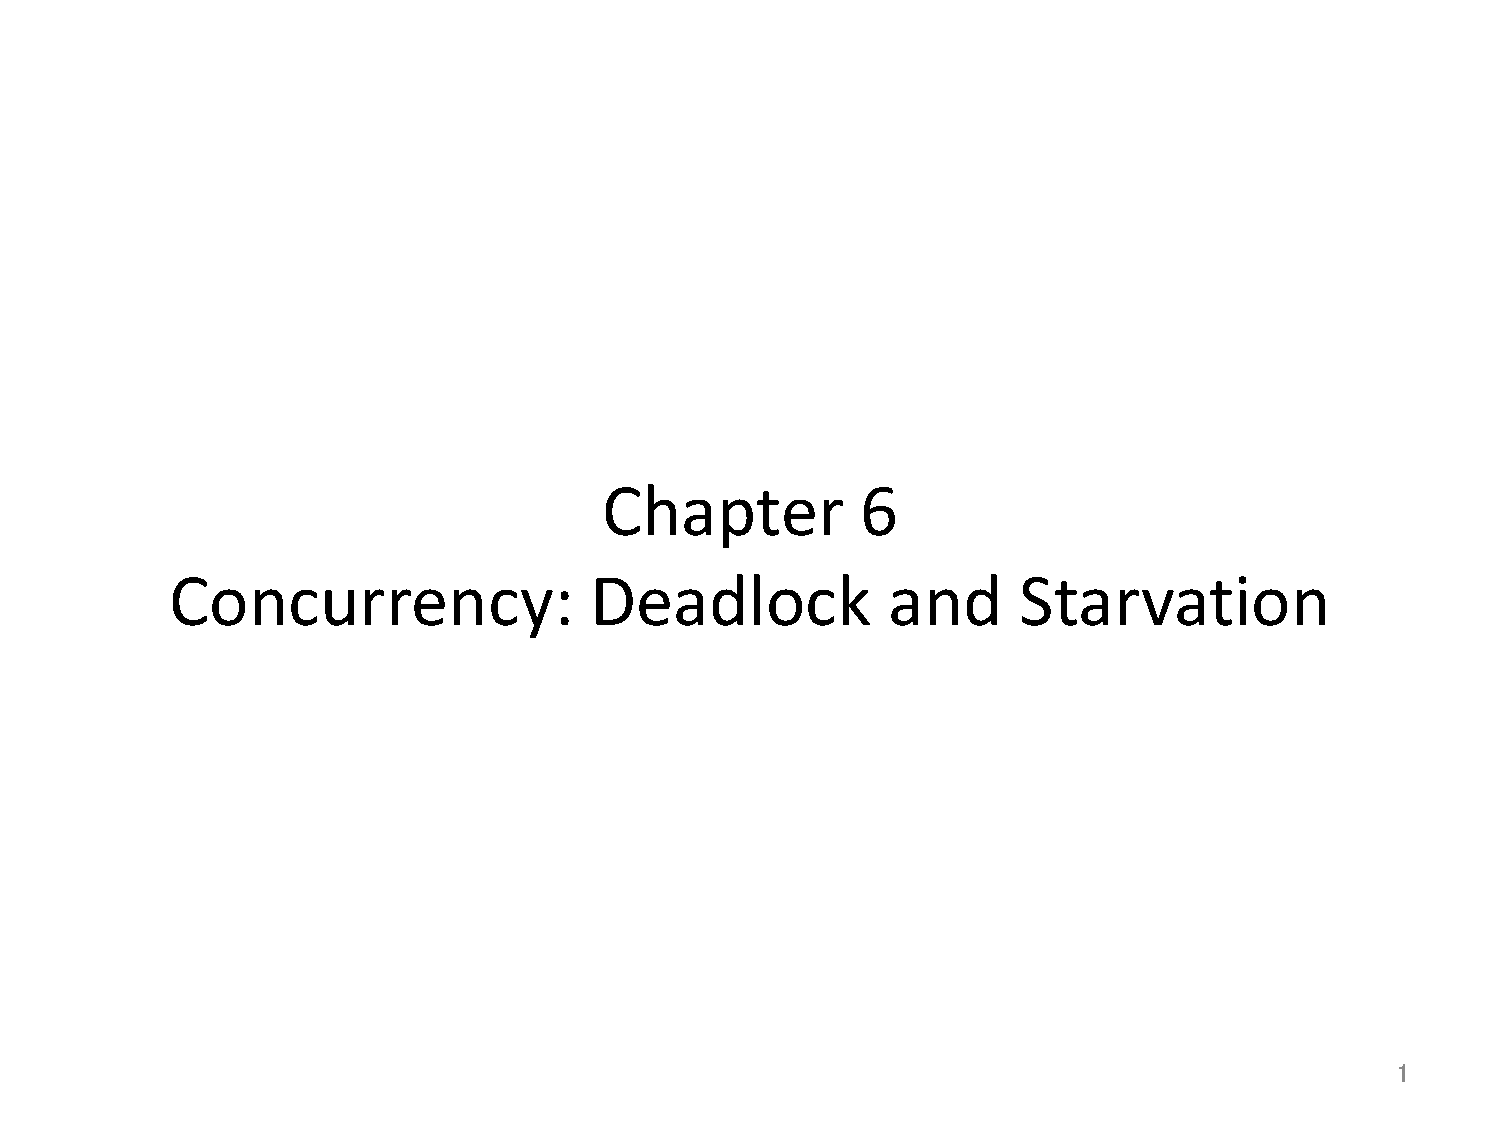
\includepdf[page=1]{06.pdf}
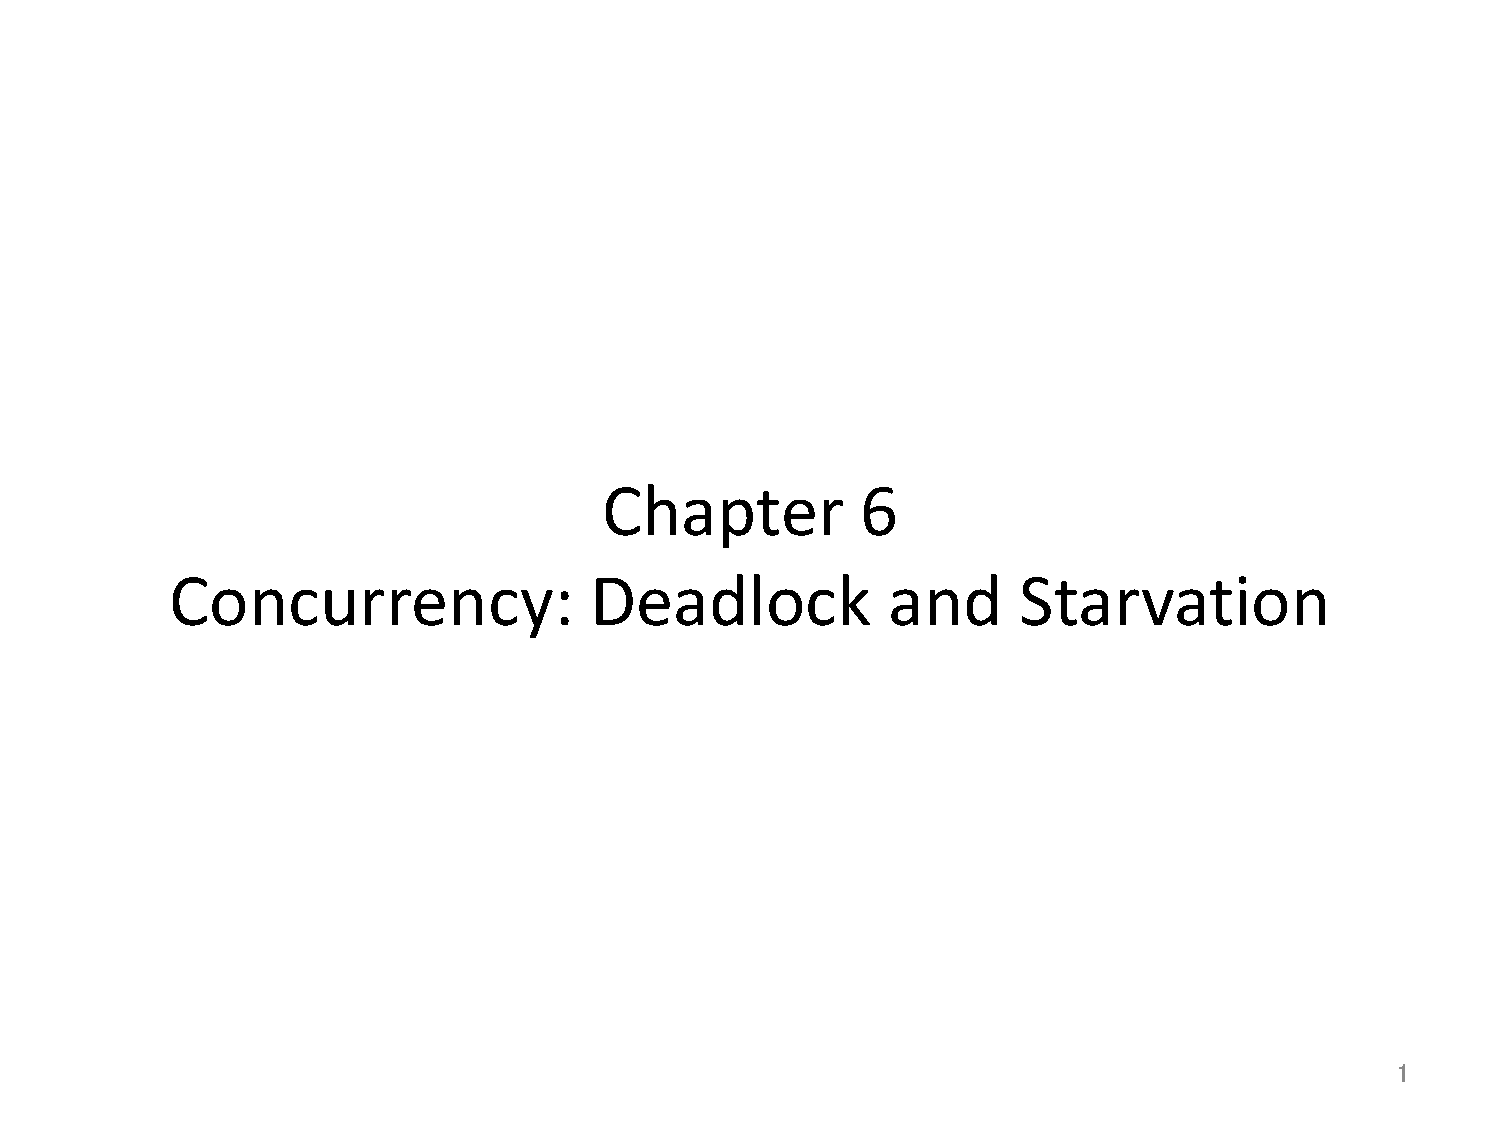
\includepdf[page=2]{06.pdf}
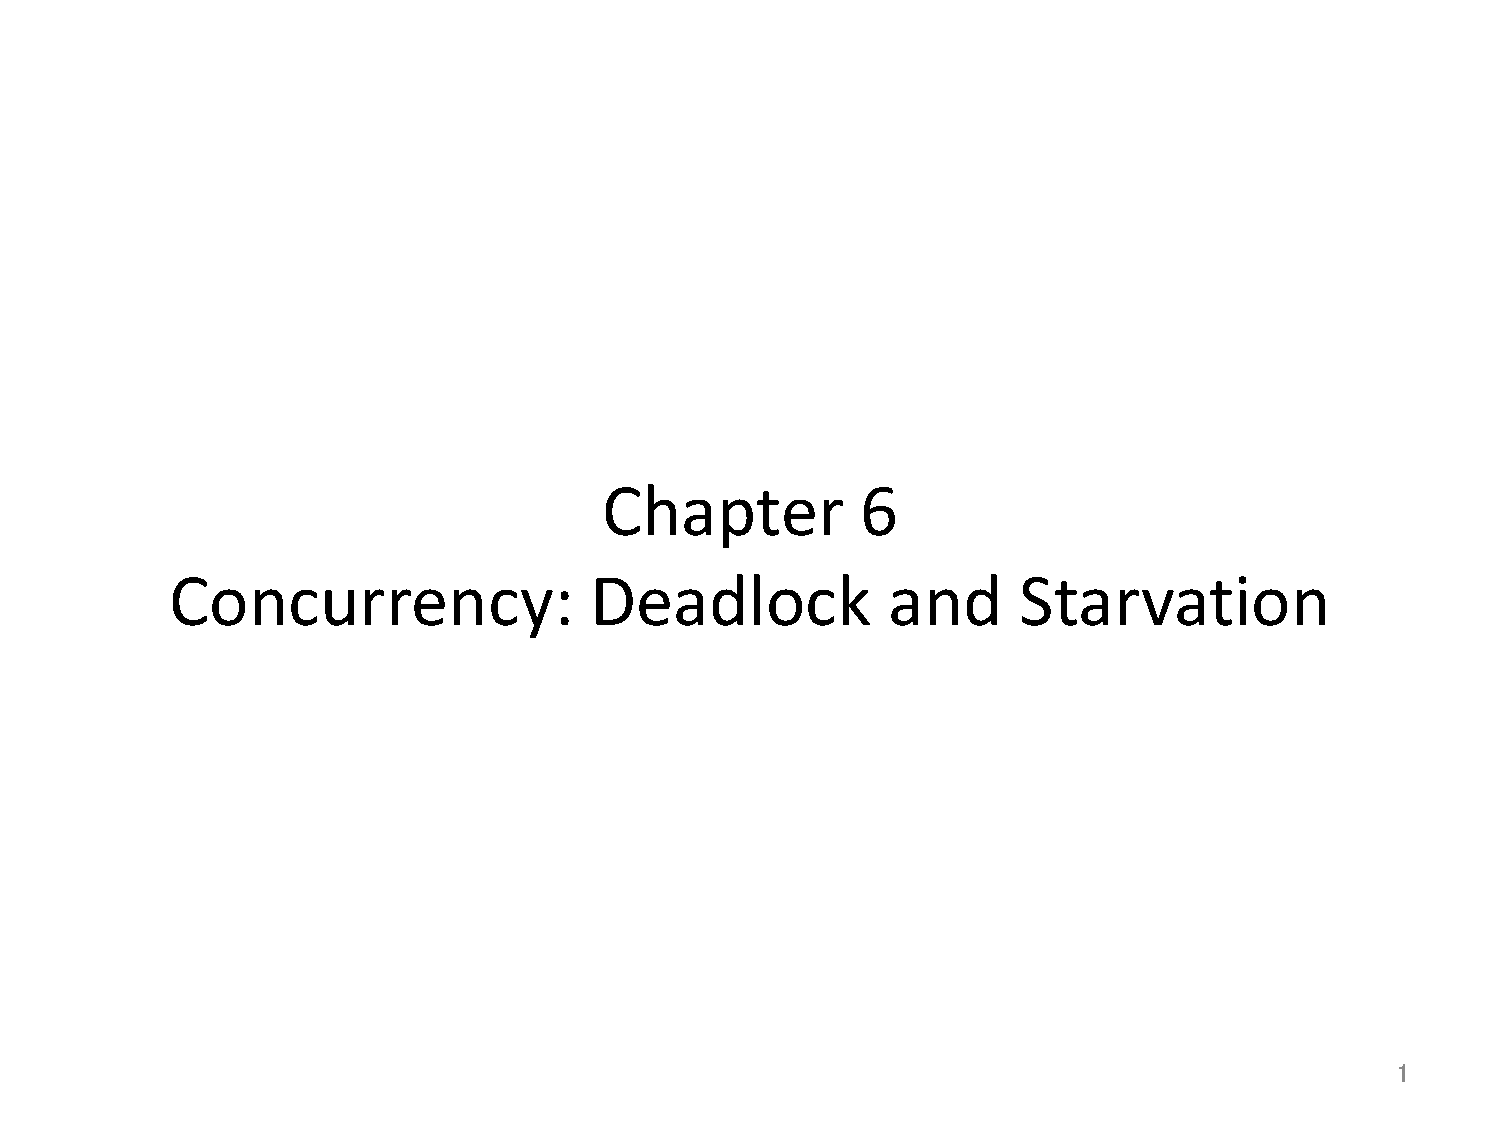
\includepdf[page=3]{06.pdf}
Lets say we have processe P and Q and two resources A and B. P calls get(A), get(B), release(A), release(B). Q calls get(B), get(A), release(B), release(A).

In the first path of execution (on a uniprocessor) we execute P so it now owns A. Then we start process Q who now owns B. So now P is stuck waiting on Q to release B who is stuck waiting for P to release A. Ahhhhhh deadlock nooo.

Note: this graph is odd, axis ticks are lines to execute and arrows are paths of execution.

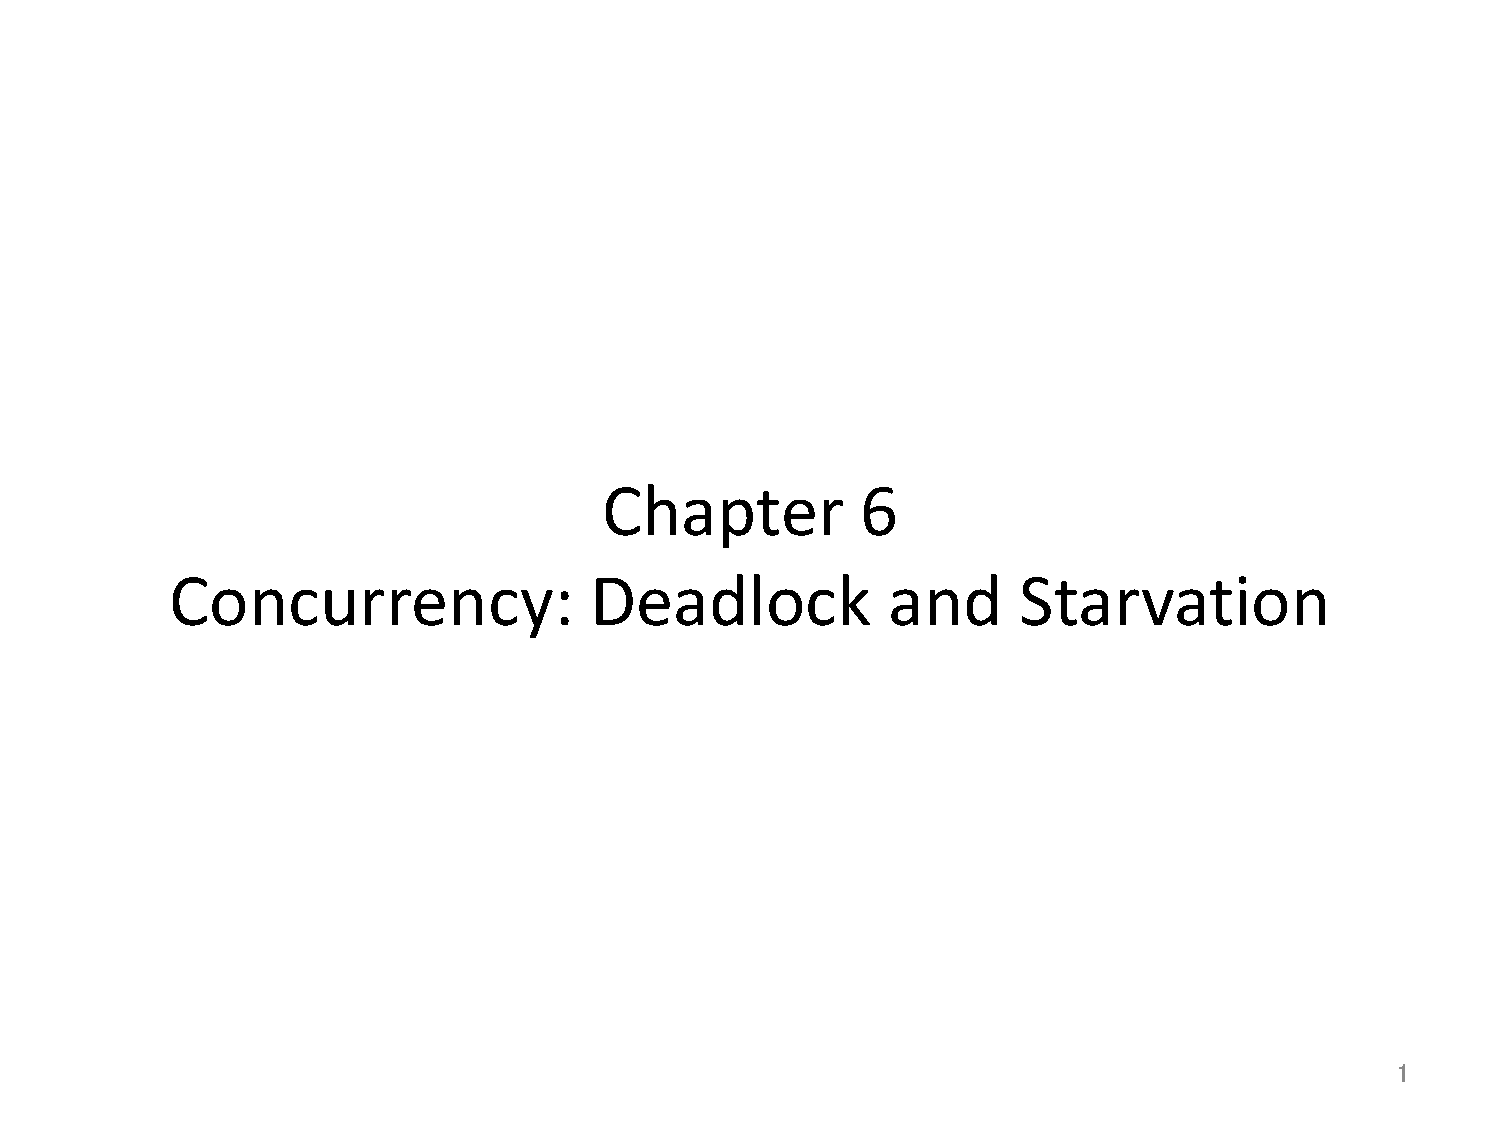
\includepdf[page=4]{06.pdf}
A way to get around this is to just attempt to avoid deadlocks in the first place. Think about the order of resource use to design it so that no one has a hold and wait situation. In this case no consecutive get commands.

Better would be for P to get(A), release(A), get(B), release(B) and do the same thing on process Q.
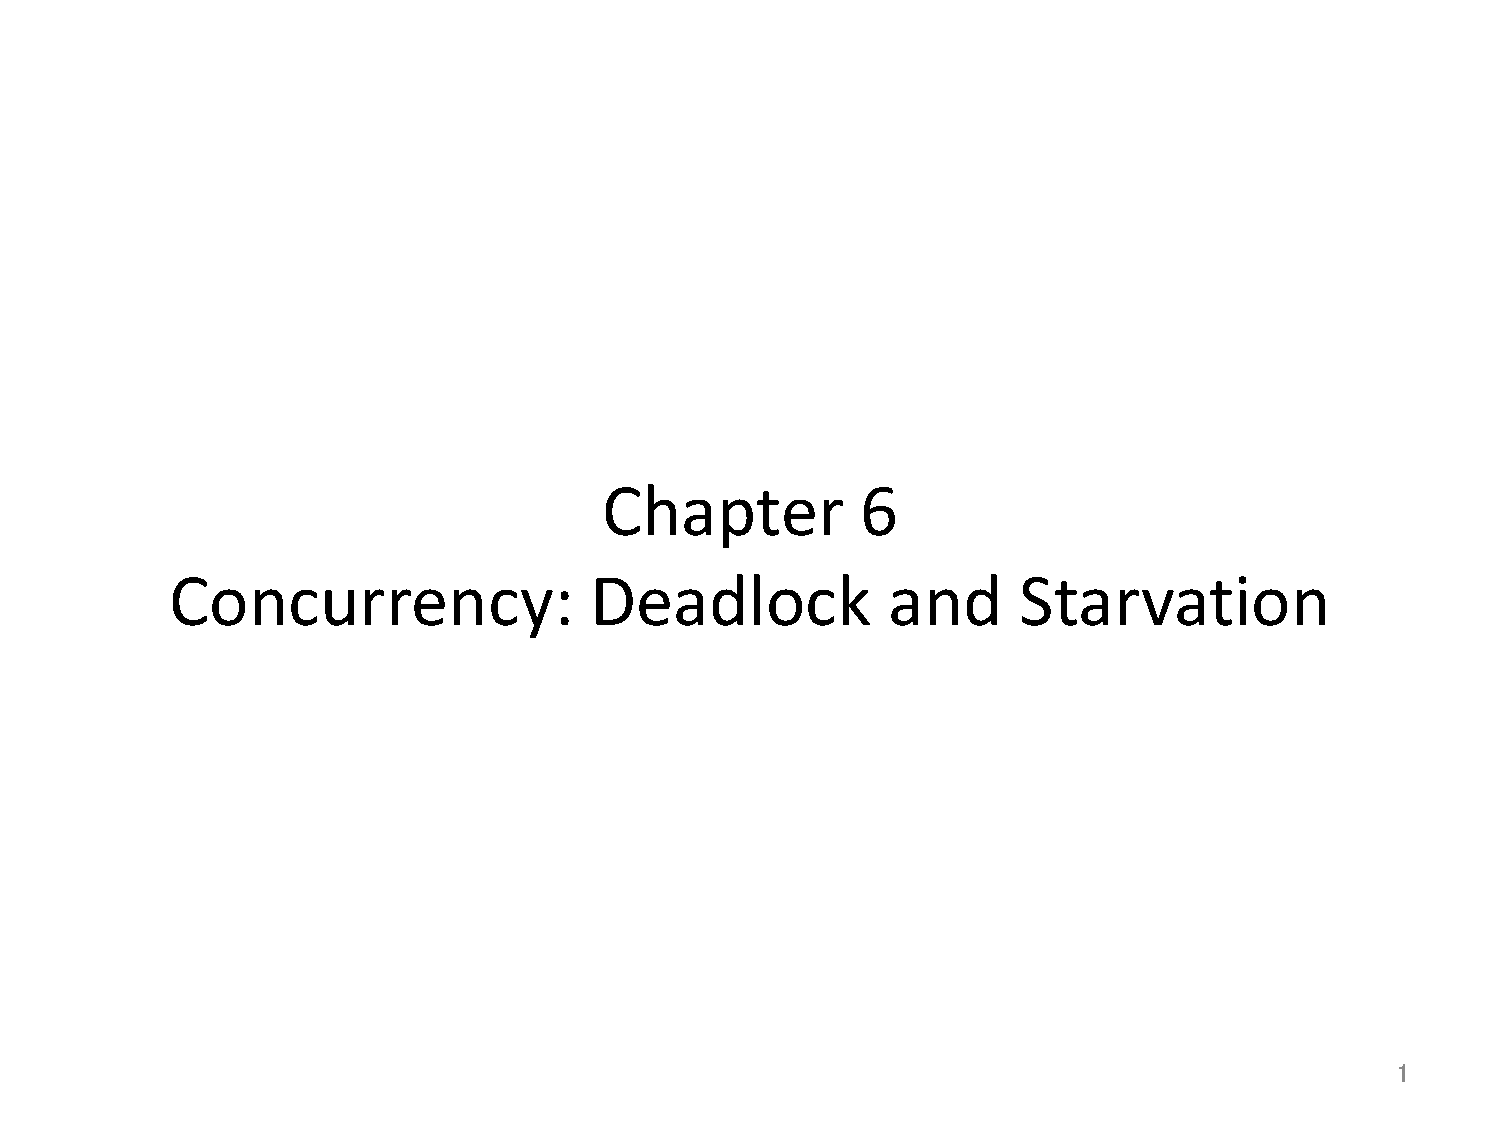
\includepdf[page=5]{06.pdf}
There are two types of resources to be blocked on, reusable and consumable.

Reusable: IO, main and secondary memory, devices, data structures. Dead lock occurs if each processn holds and then requests, only one element exists
Consumable: created and destroyed elements. Deadlock occurs if receive signal is blocked.
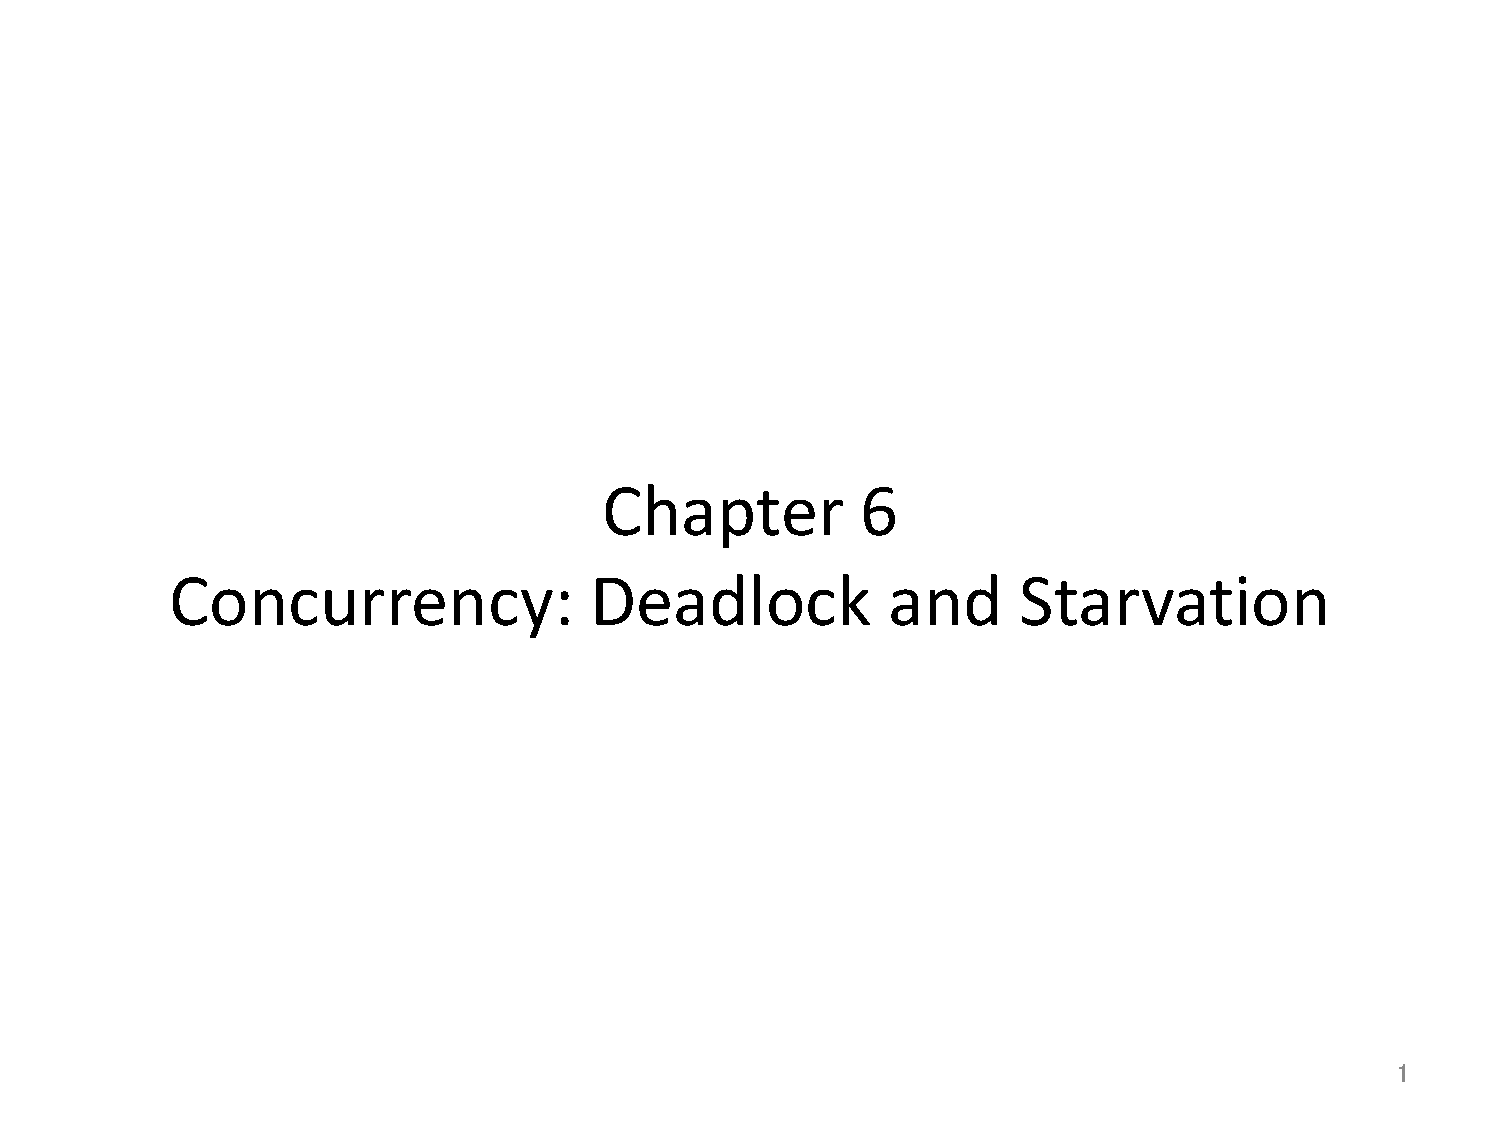
\includepdf[page=6]{06.pdf}
These are just resources that dont go away as you use them. These you have to release before you request again if you want assurance that a deadlock wont occur.

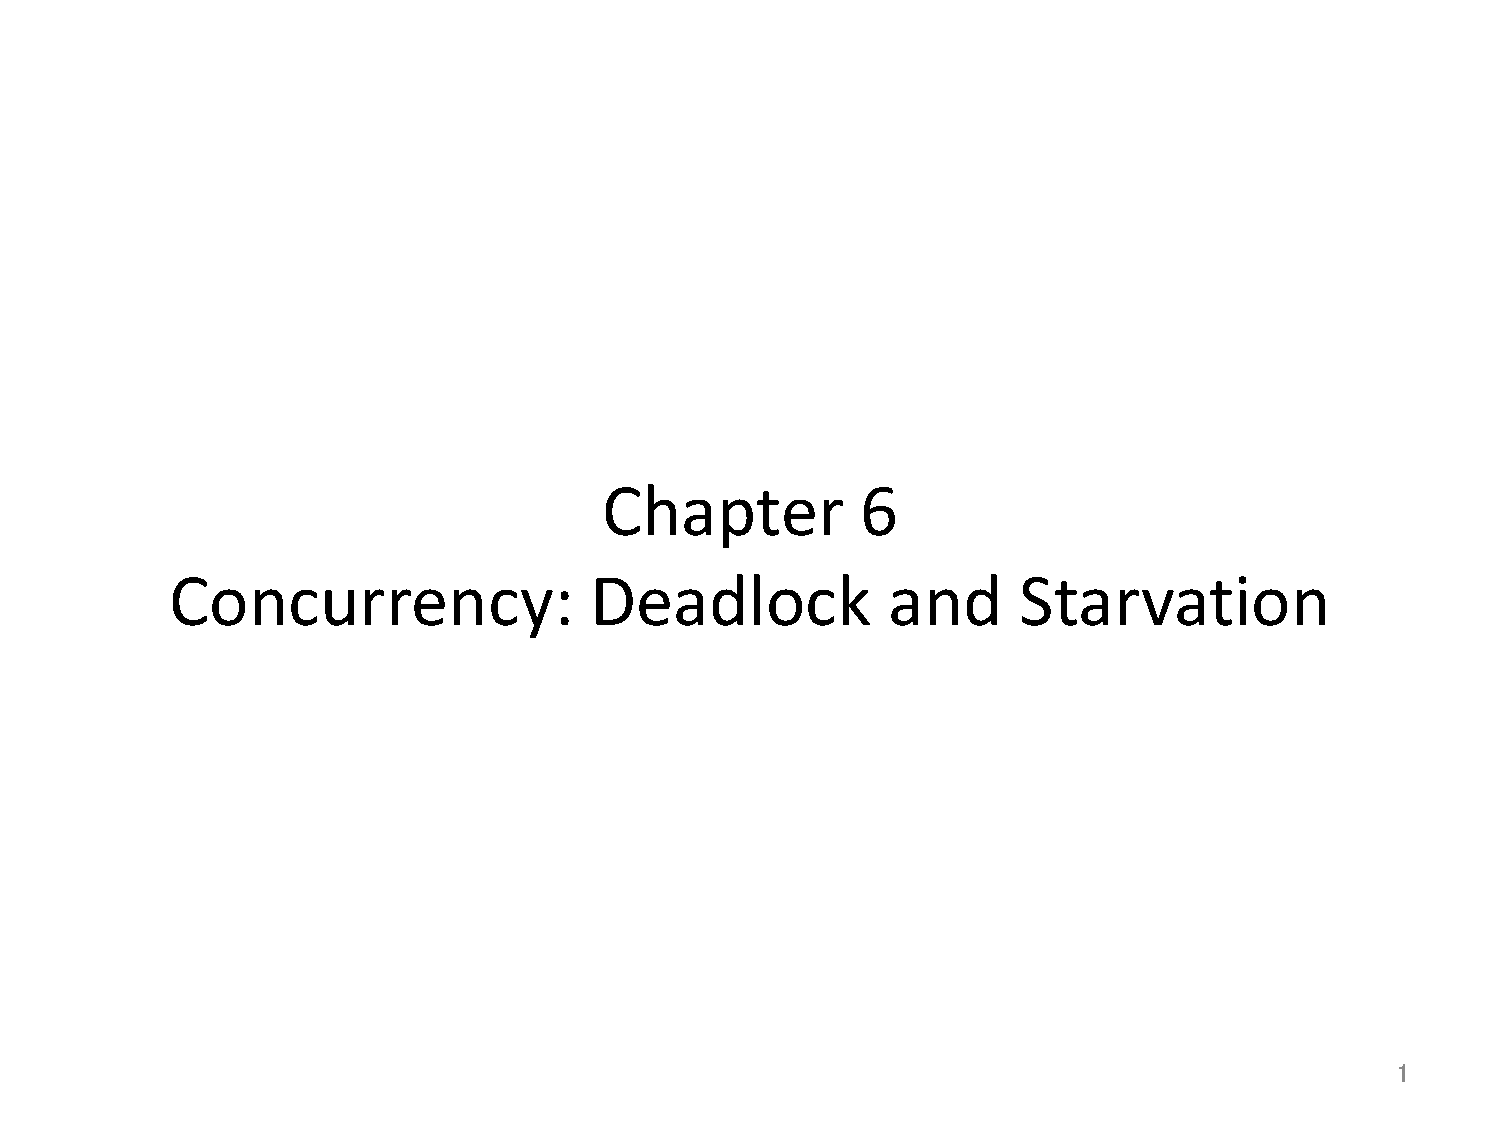
\includepdf[page=7]{06.pdf}
In this example we run out of memory no matter the order of execution.
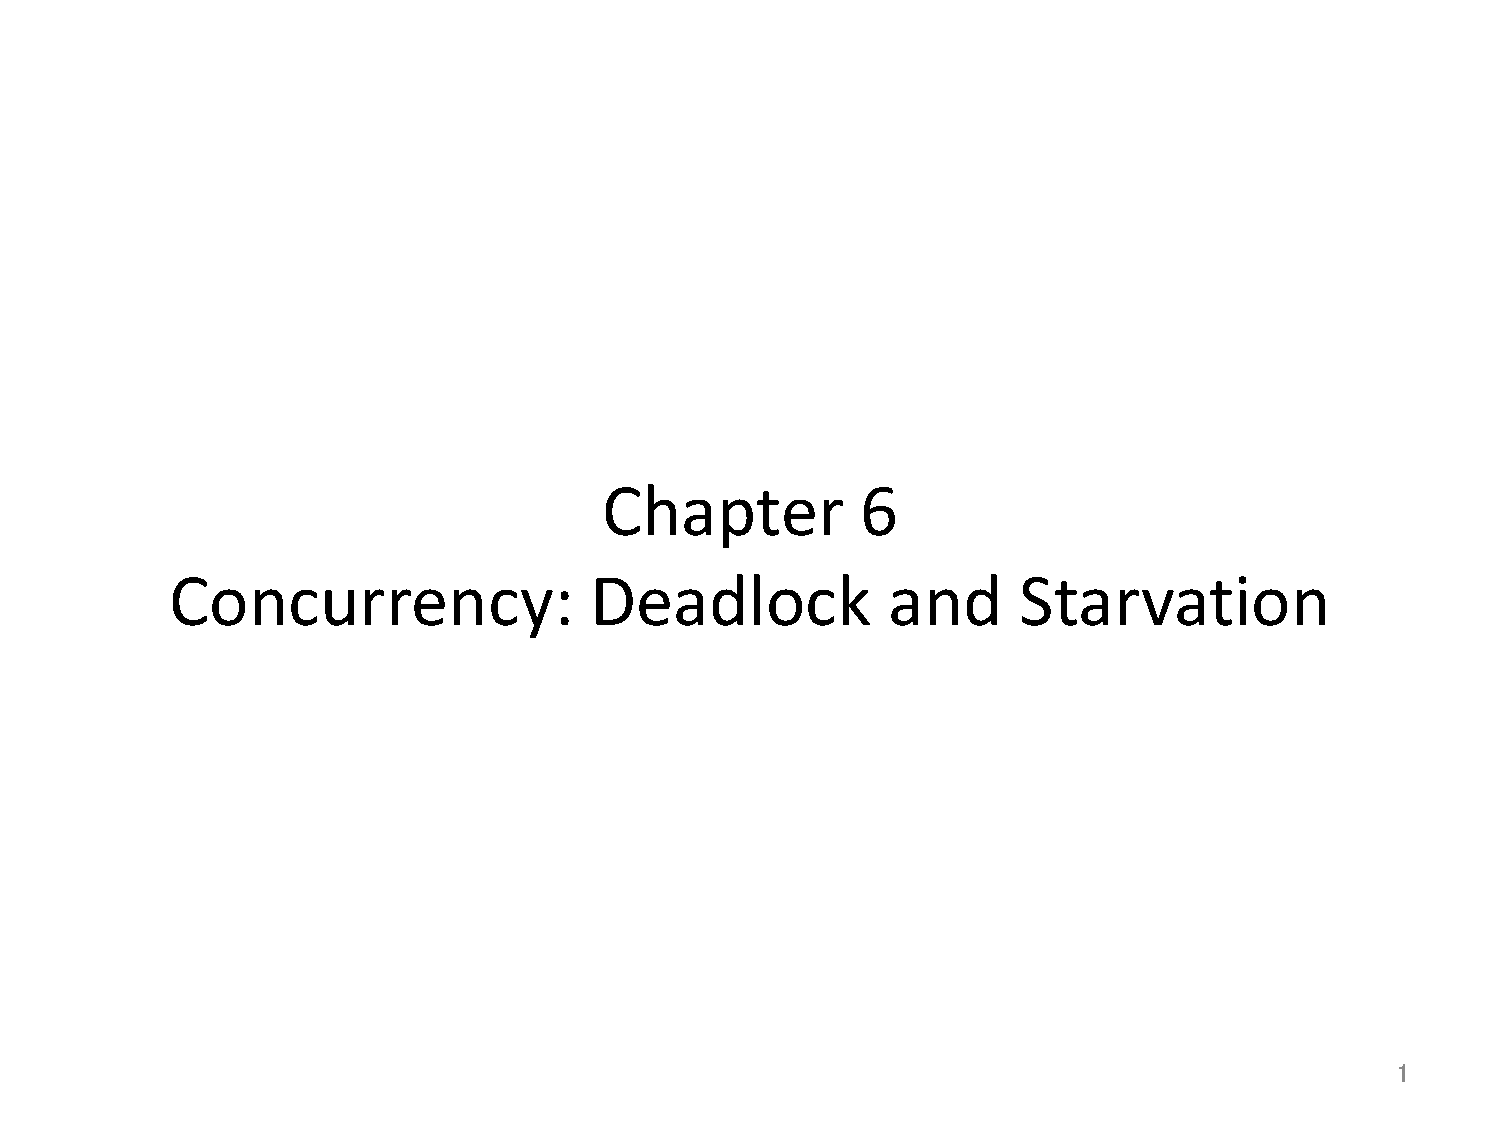
\includepdf[page=8]{06.pdf}
Here is an example of message passing. If each message queue is empty we have a deadlock because neither program can reach the point at which they send the message.
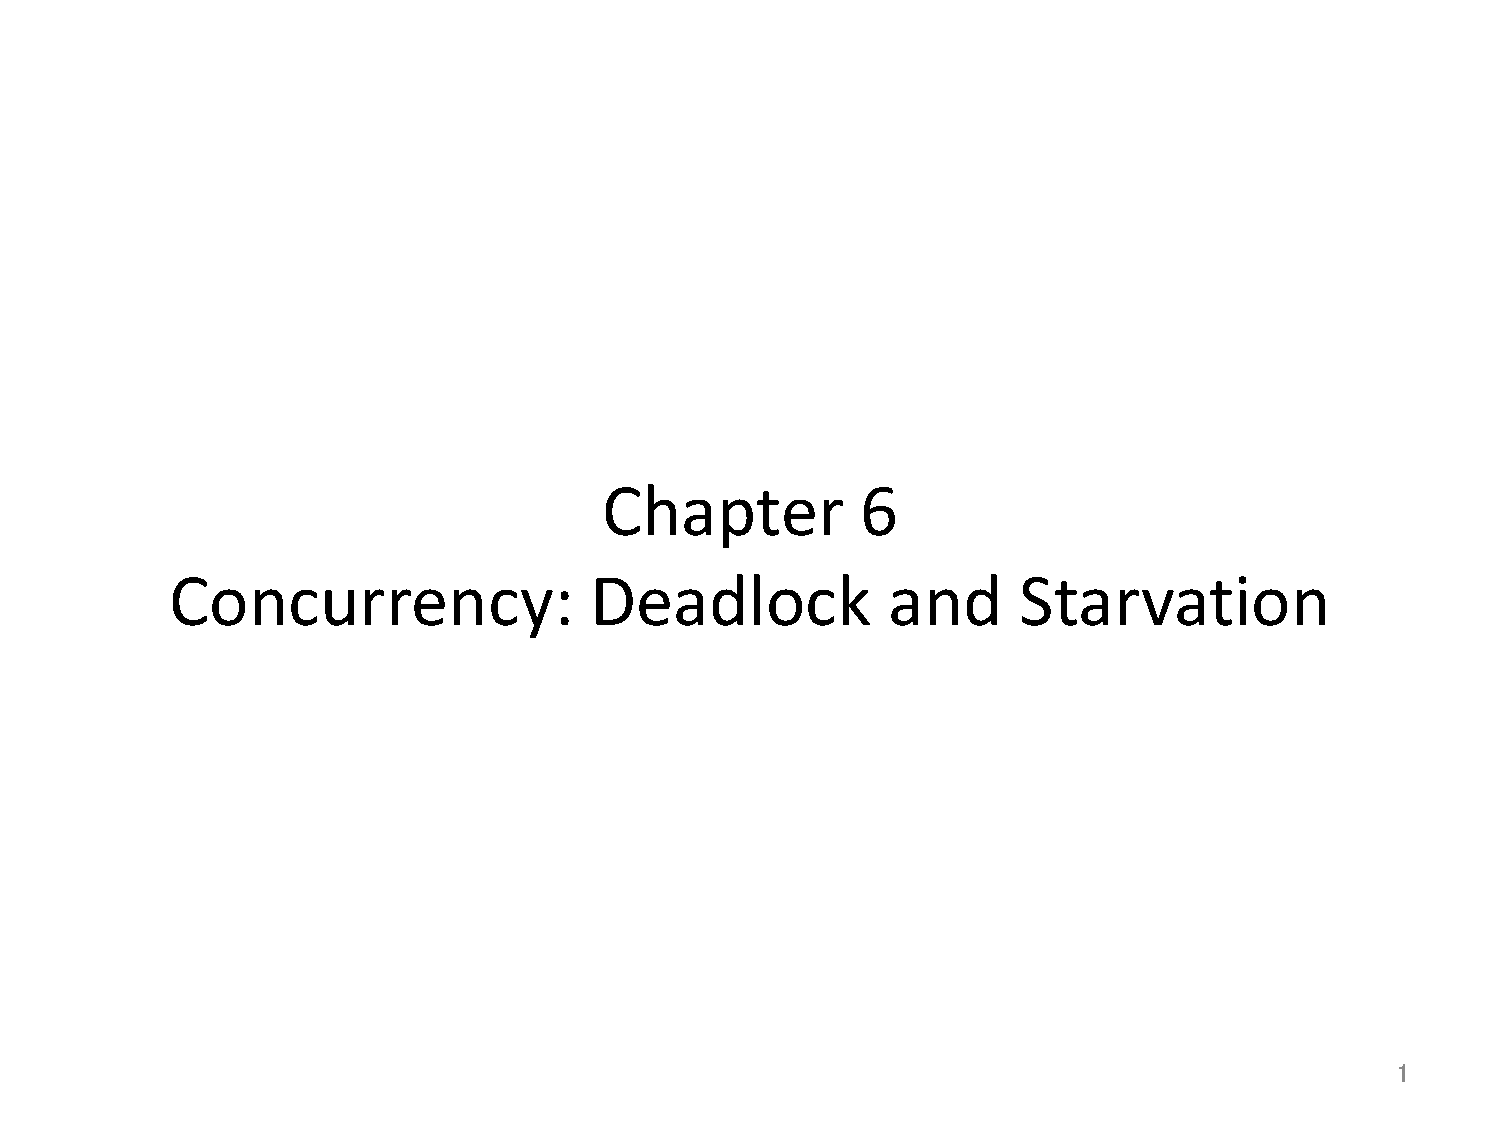
\includepdf[page=9]{06.pdf}
Squares are resources and circles are processes.
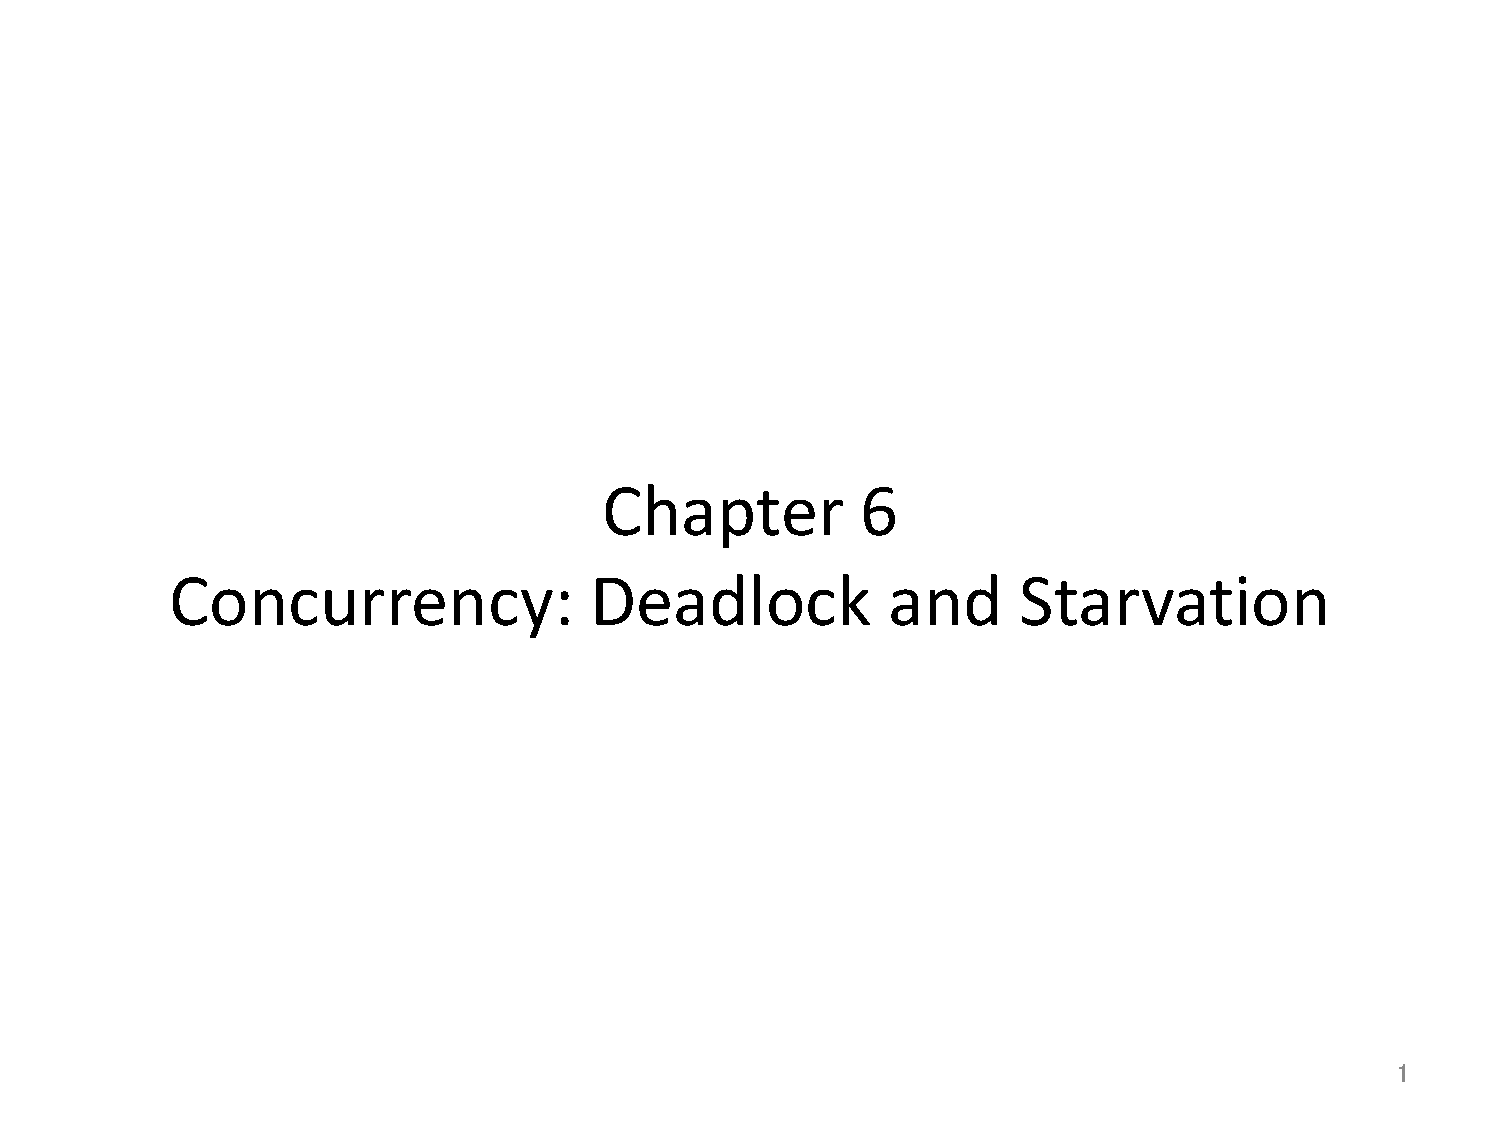
\includepdf[page=10]{06.pdf}
Mutual exclusion is the cause of deadlocks since we block on resources, if we dont have mutual exclusion everyone just accesses willy nilly. Deadlocks also need to have a instance where a process holds onto a resource for more than one cycle to give other processes time to attempt to get it. We also need to not have preemption of resource so we cannot force an resource from an entity.
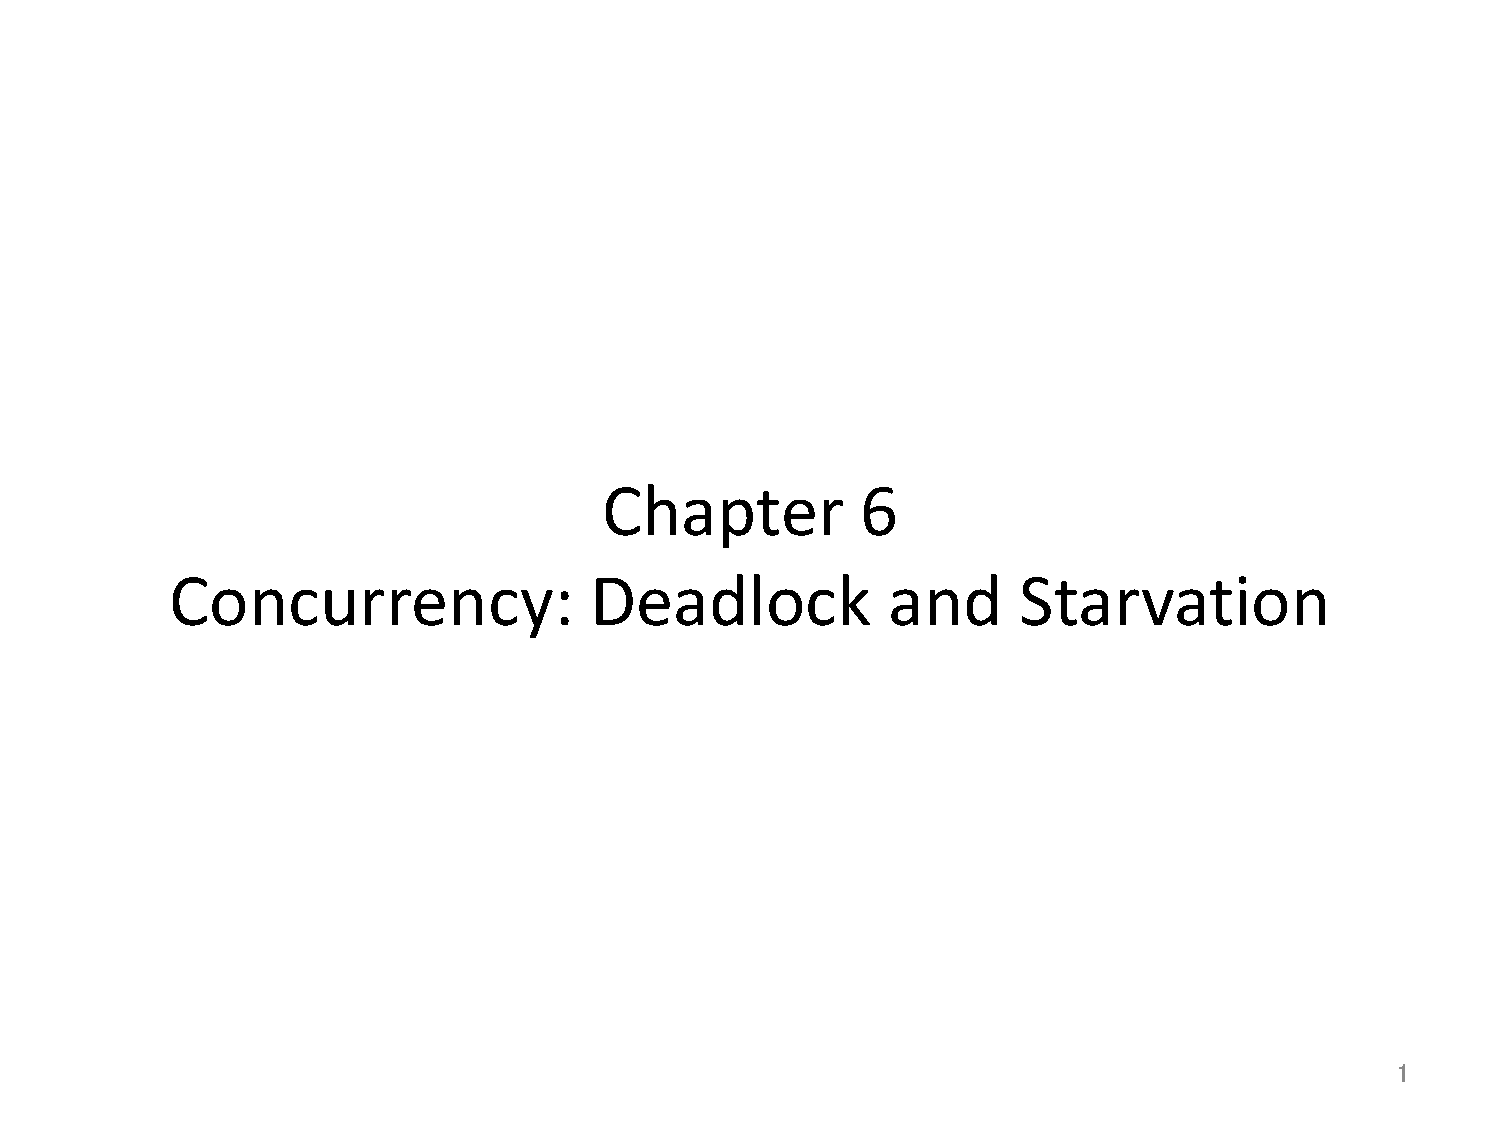
\includepdf[page=11]{06.pdf}
This is the main condition for a deadlock. One process must hold a resource that is needed by a process that holds a resource the initial process needs.

If we are missing any of the above conditions we wont get deadlocks.
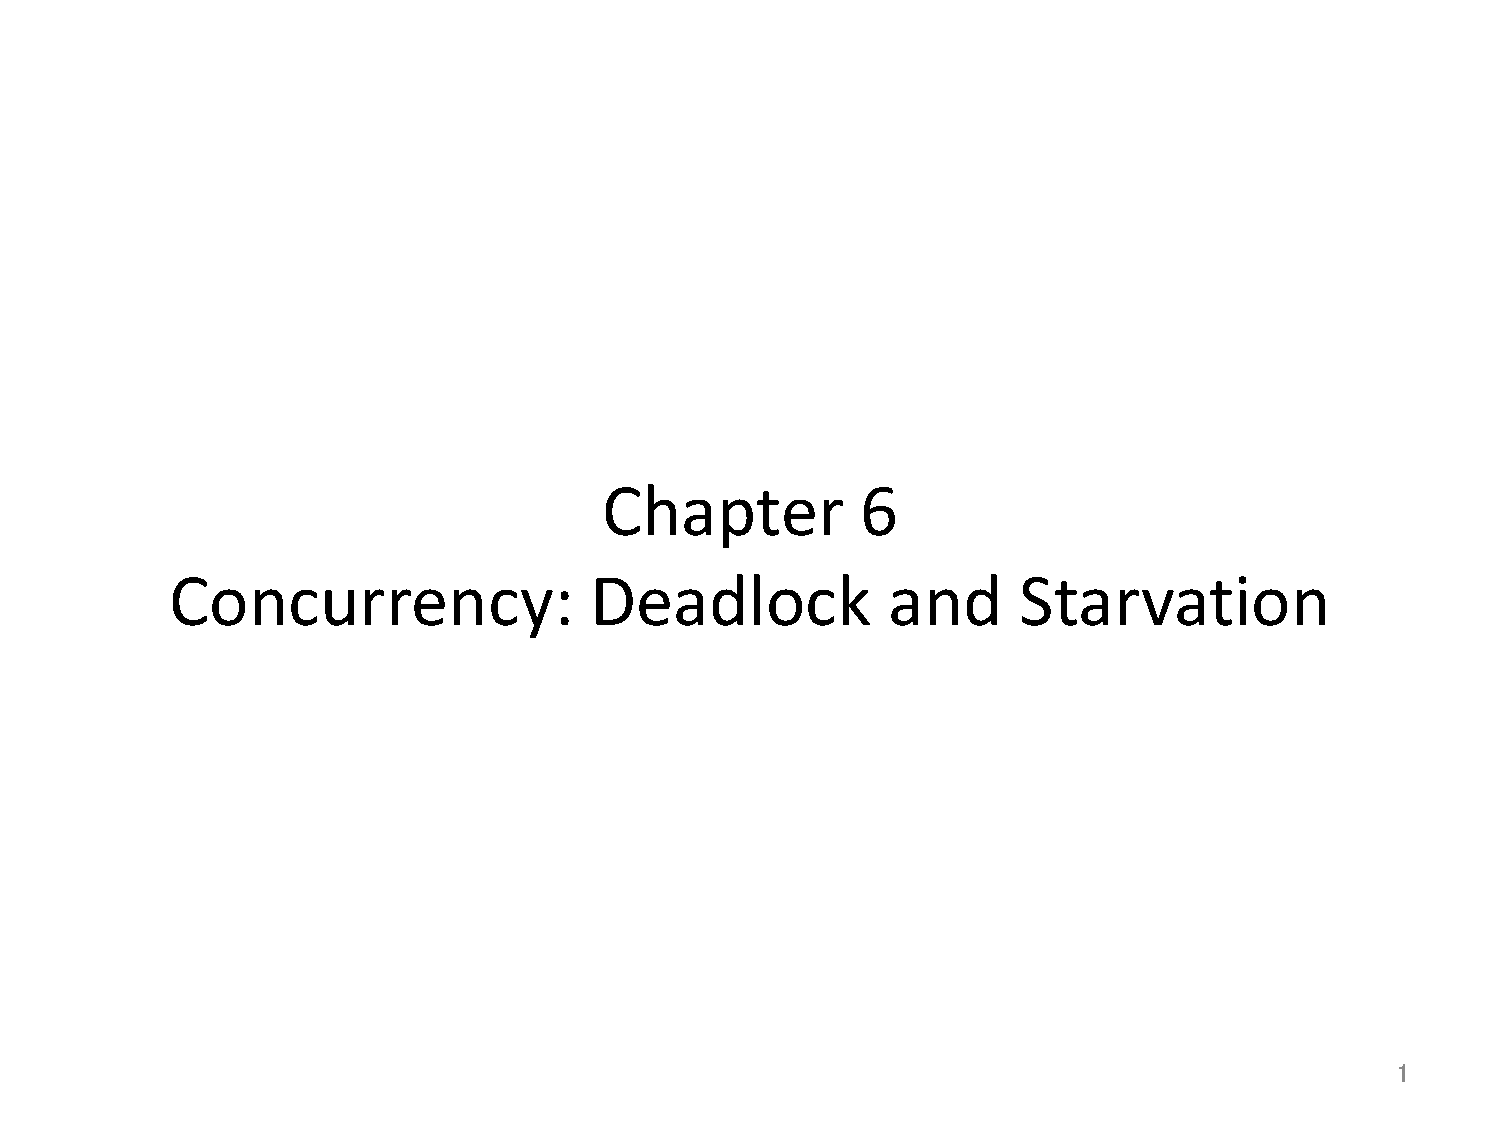
\includepdf[page=12]{06.pdf}
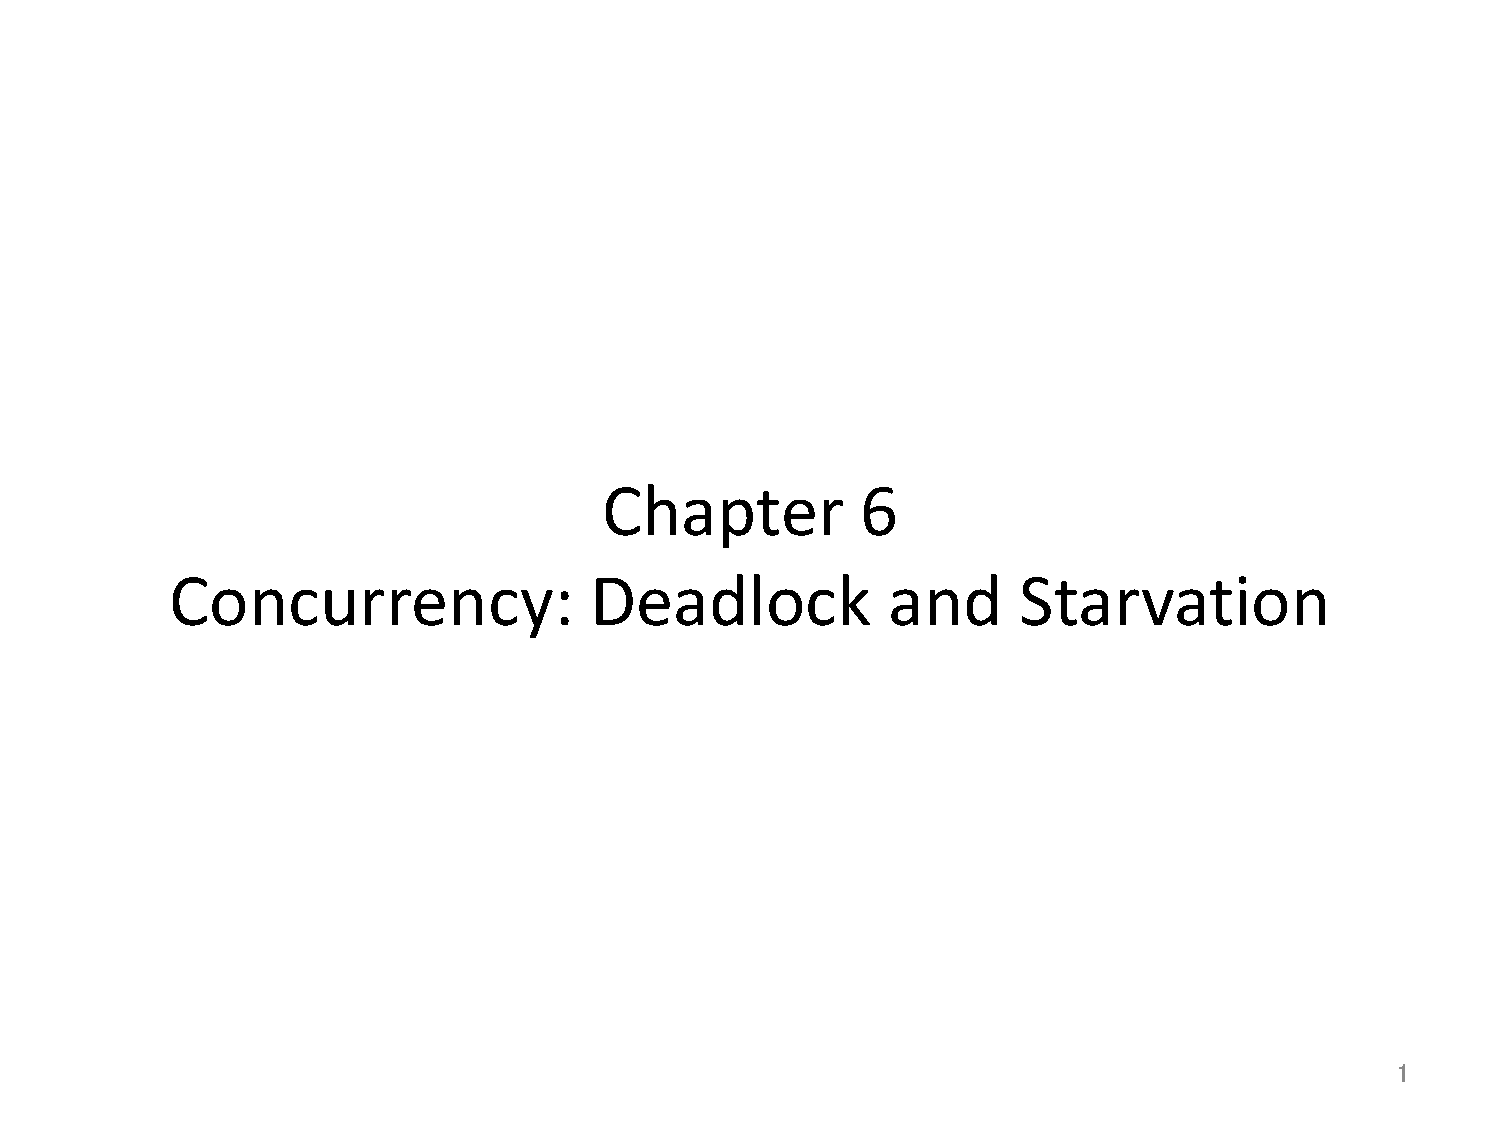
\includepdf[page=13]{06.pdf}
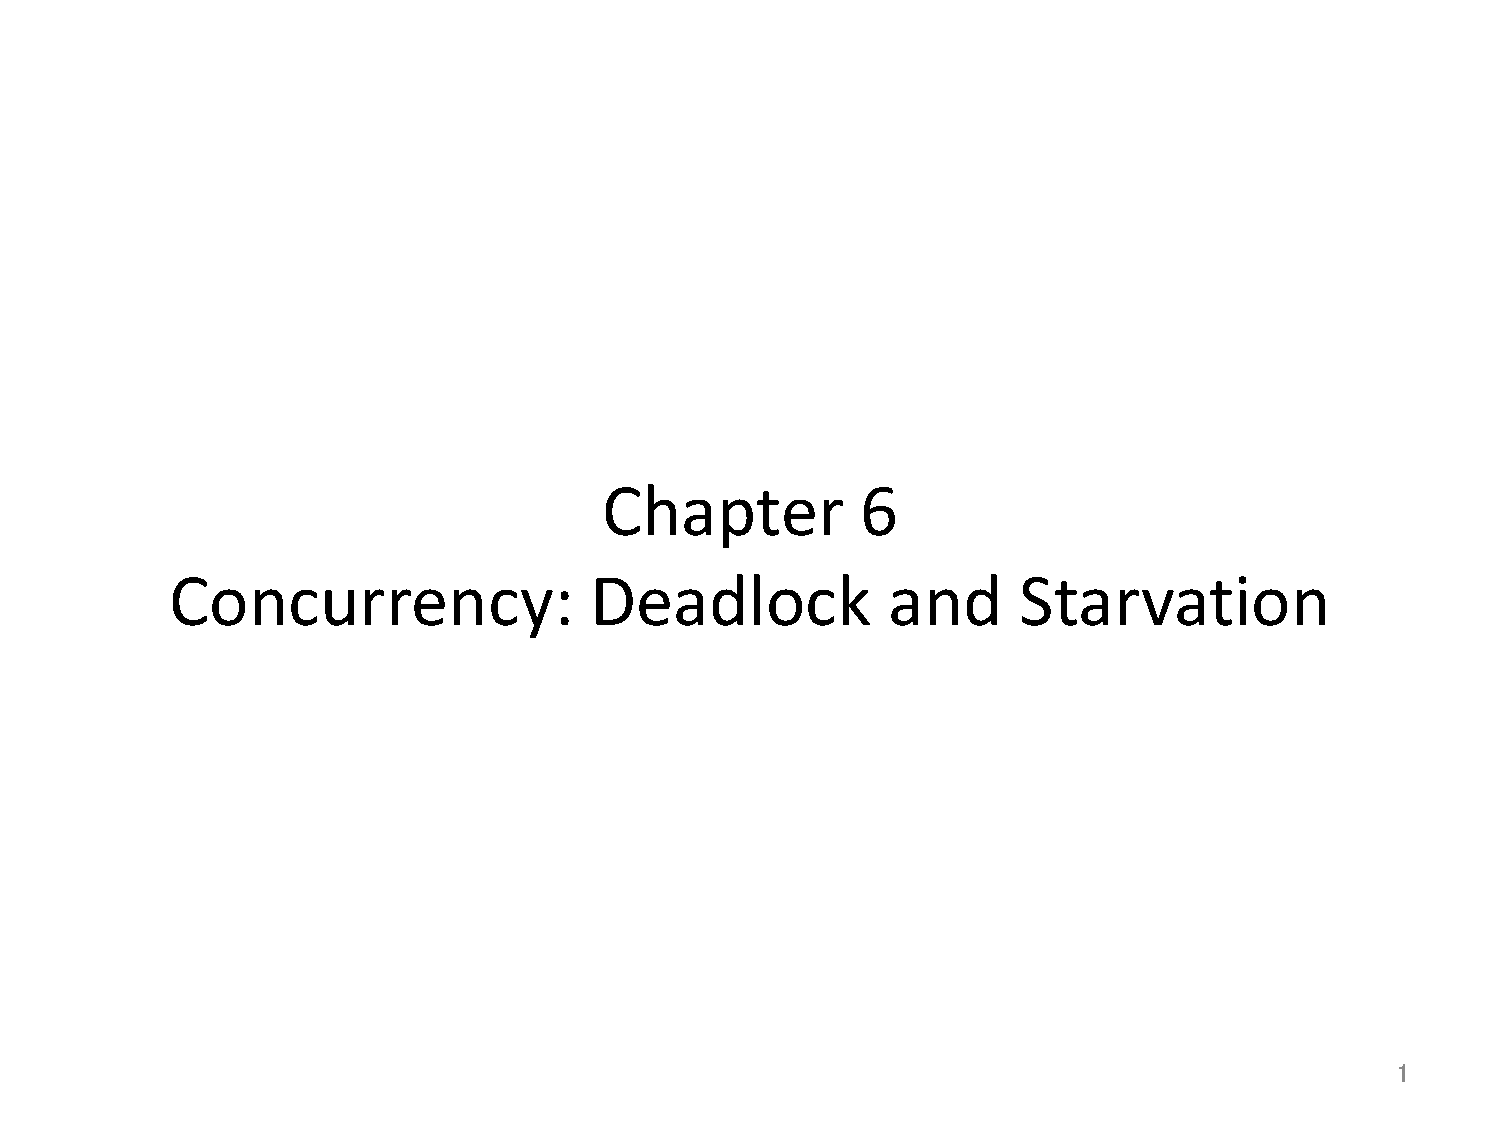
\includepdf[page=14]{06.pdf}
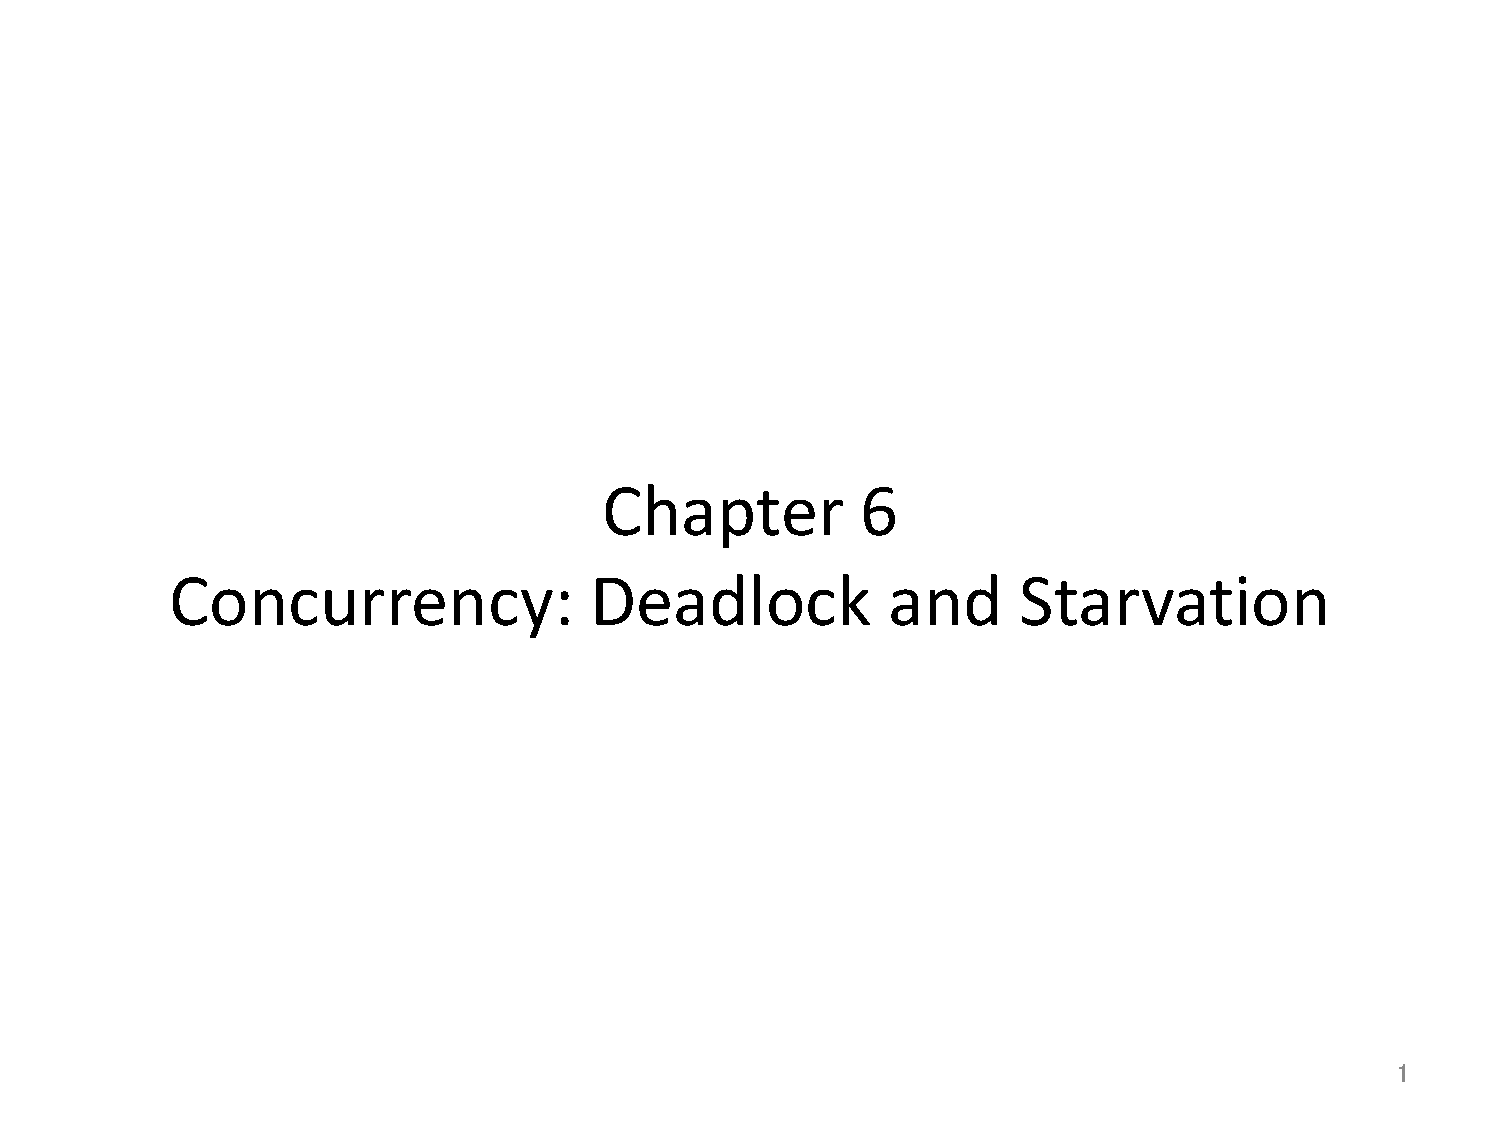
\includepdf[page=15]{06.pdf}
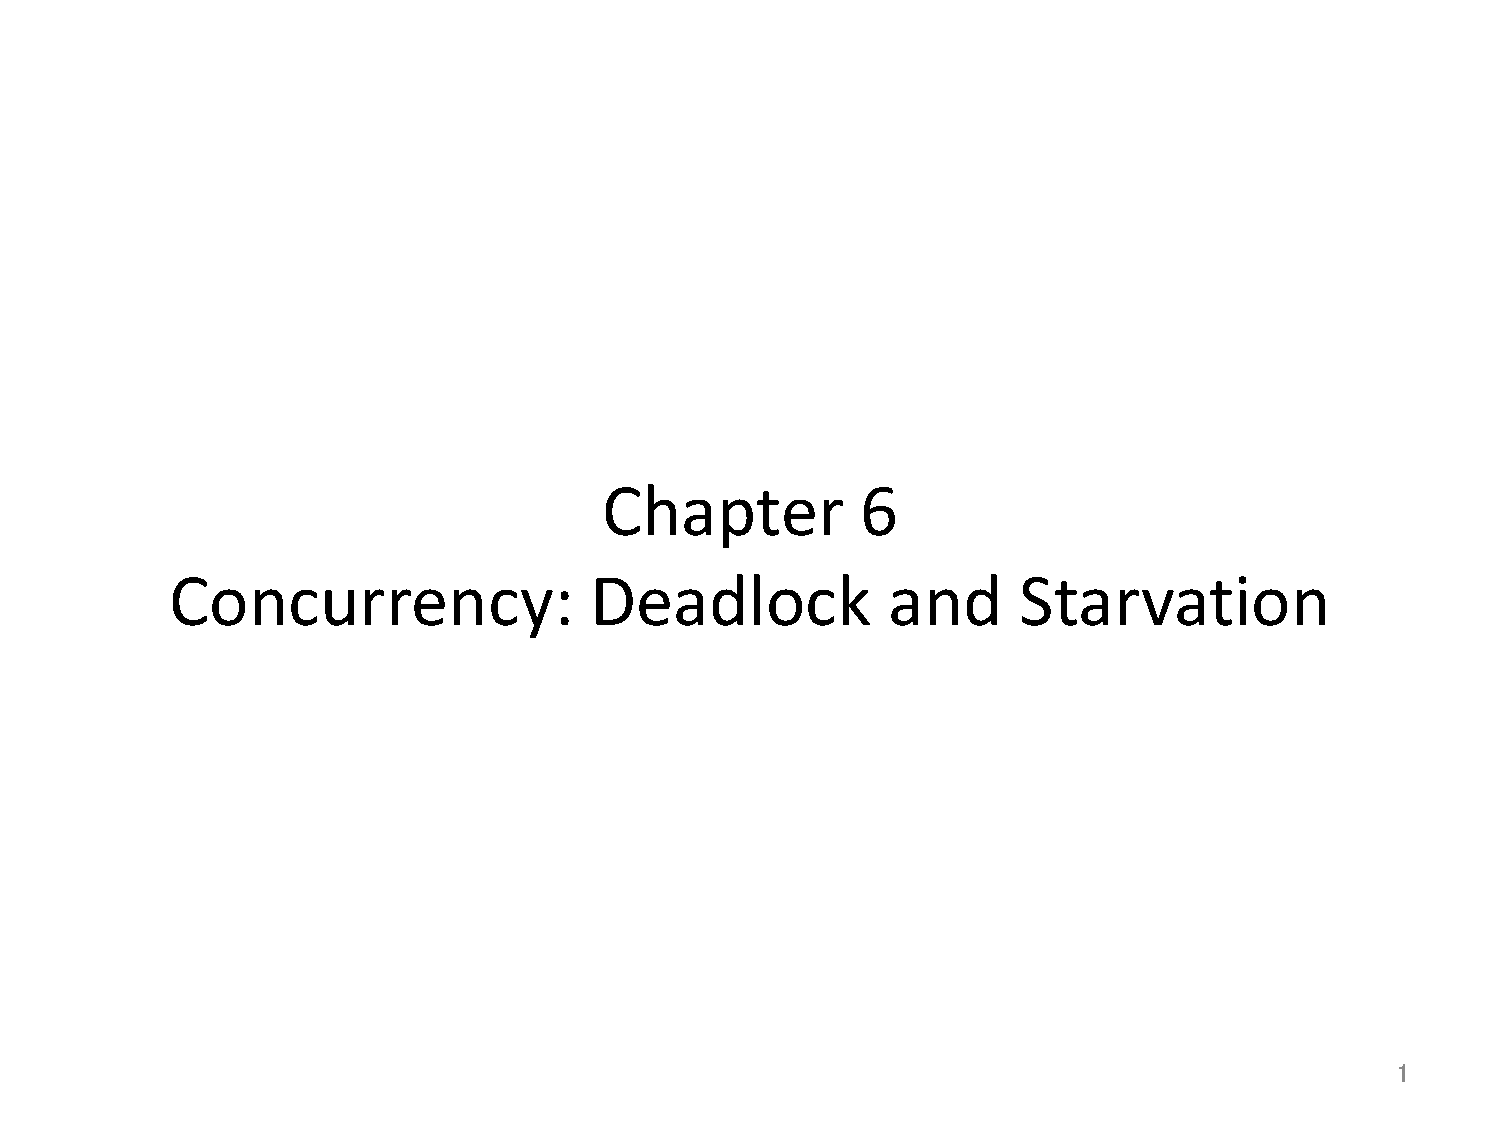
\includepdf[page=16]{06.pdf}
Hold and Wait: Try to allocate all of the resources needed at beginning. This also means that we dont waste anytime.
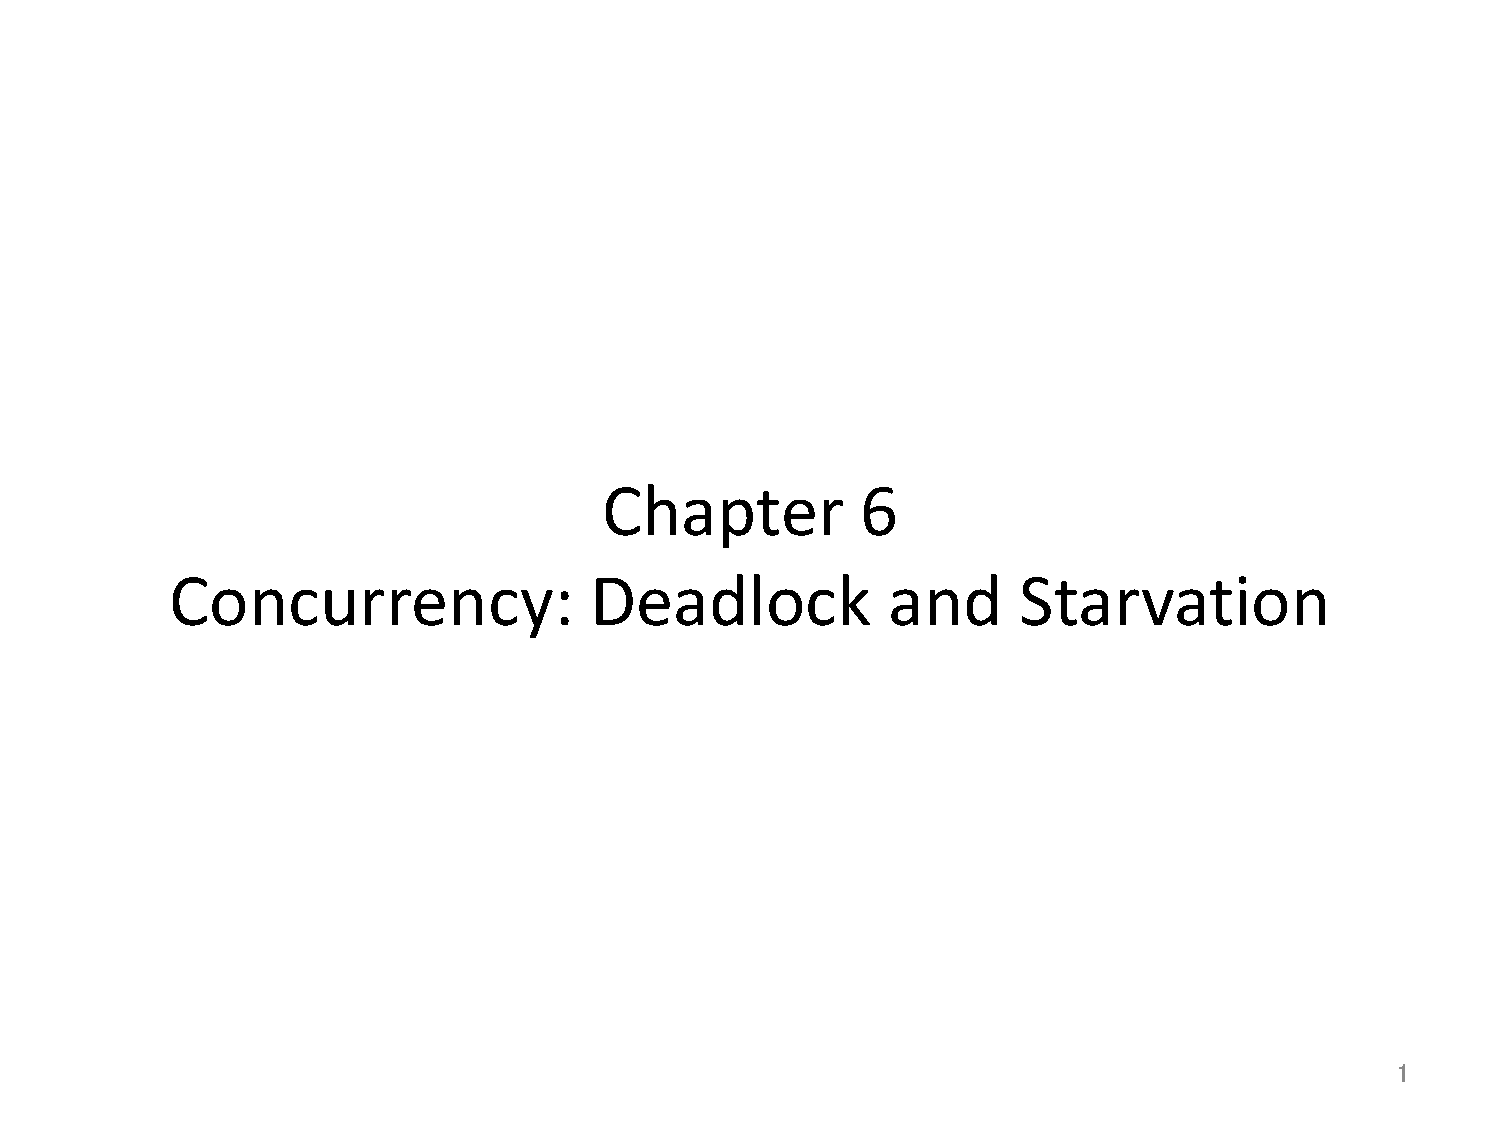
\includepdf[page=17]{06.pdf}
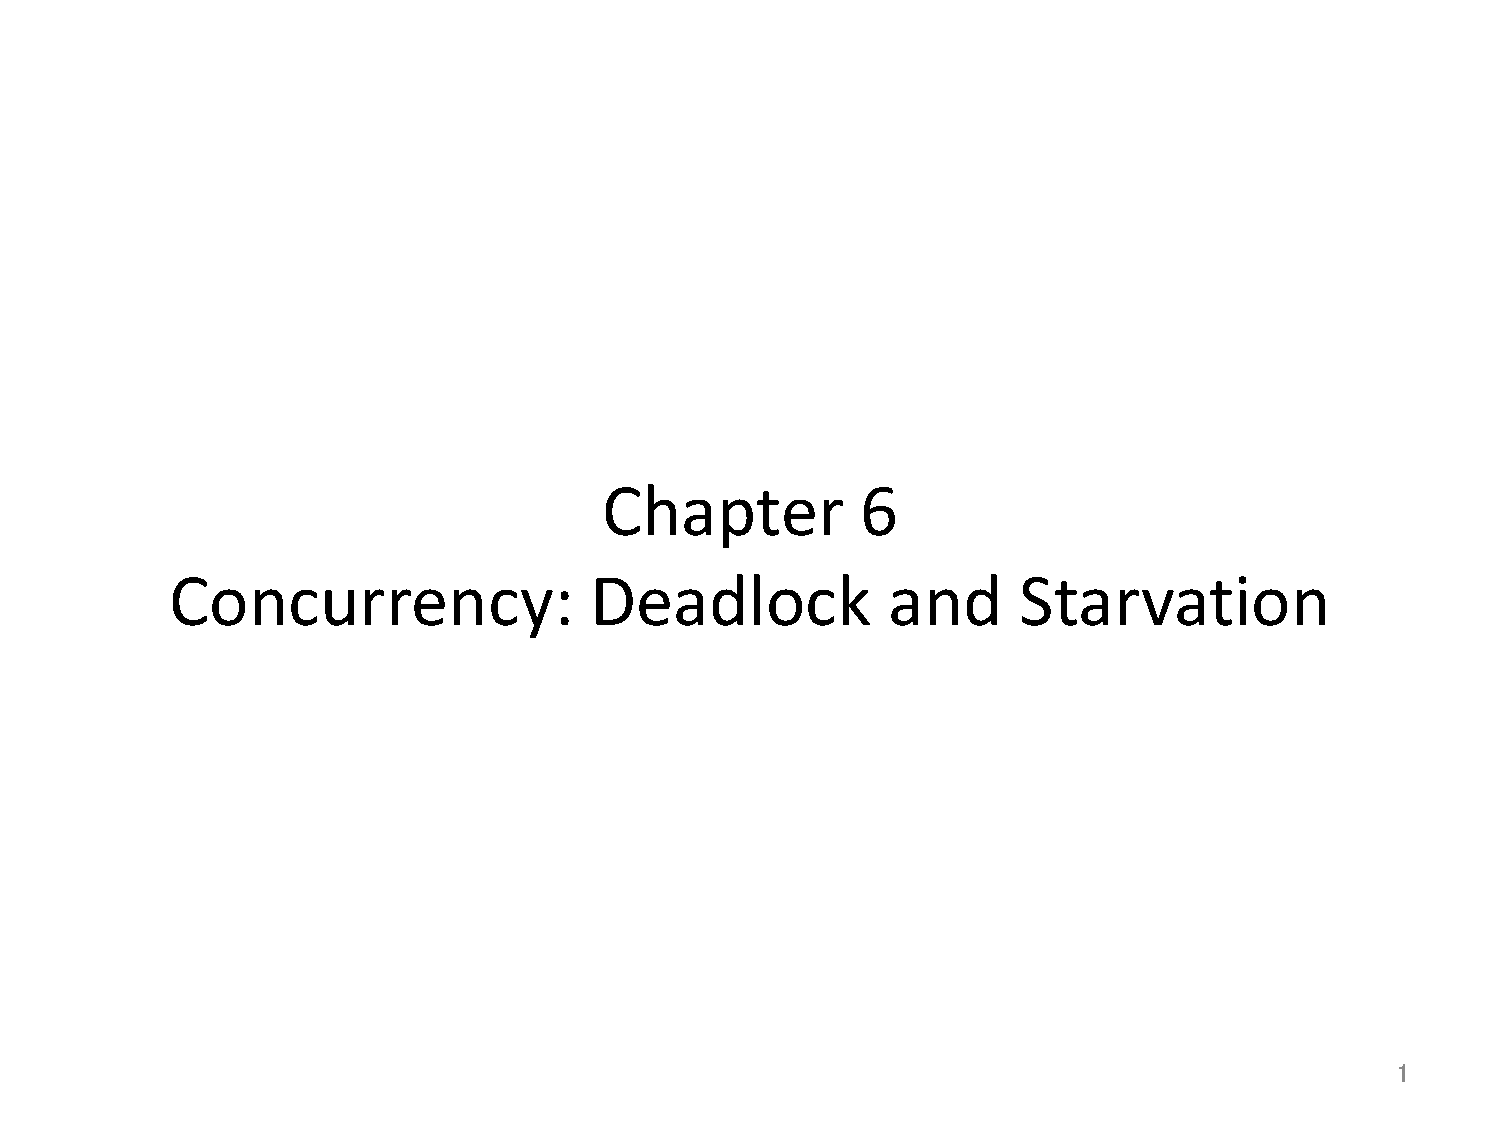
\includepdf[page=18]{06.pdf}
Instead of attacking crude assumptions we try to make descisions at runtime. Banker's algorithm avoids incremental requests for resource allocation is an example of one such algorithm
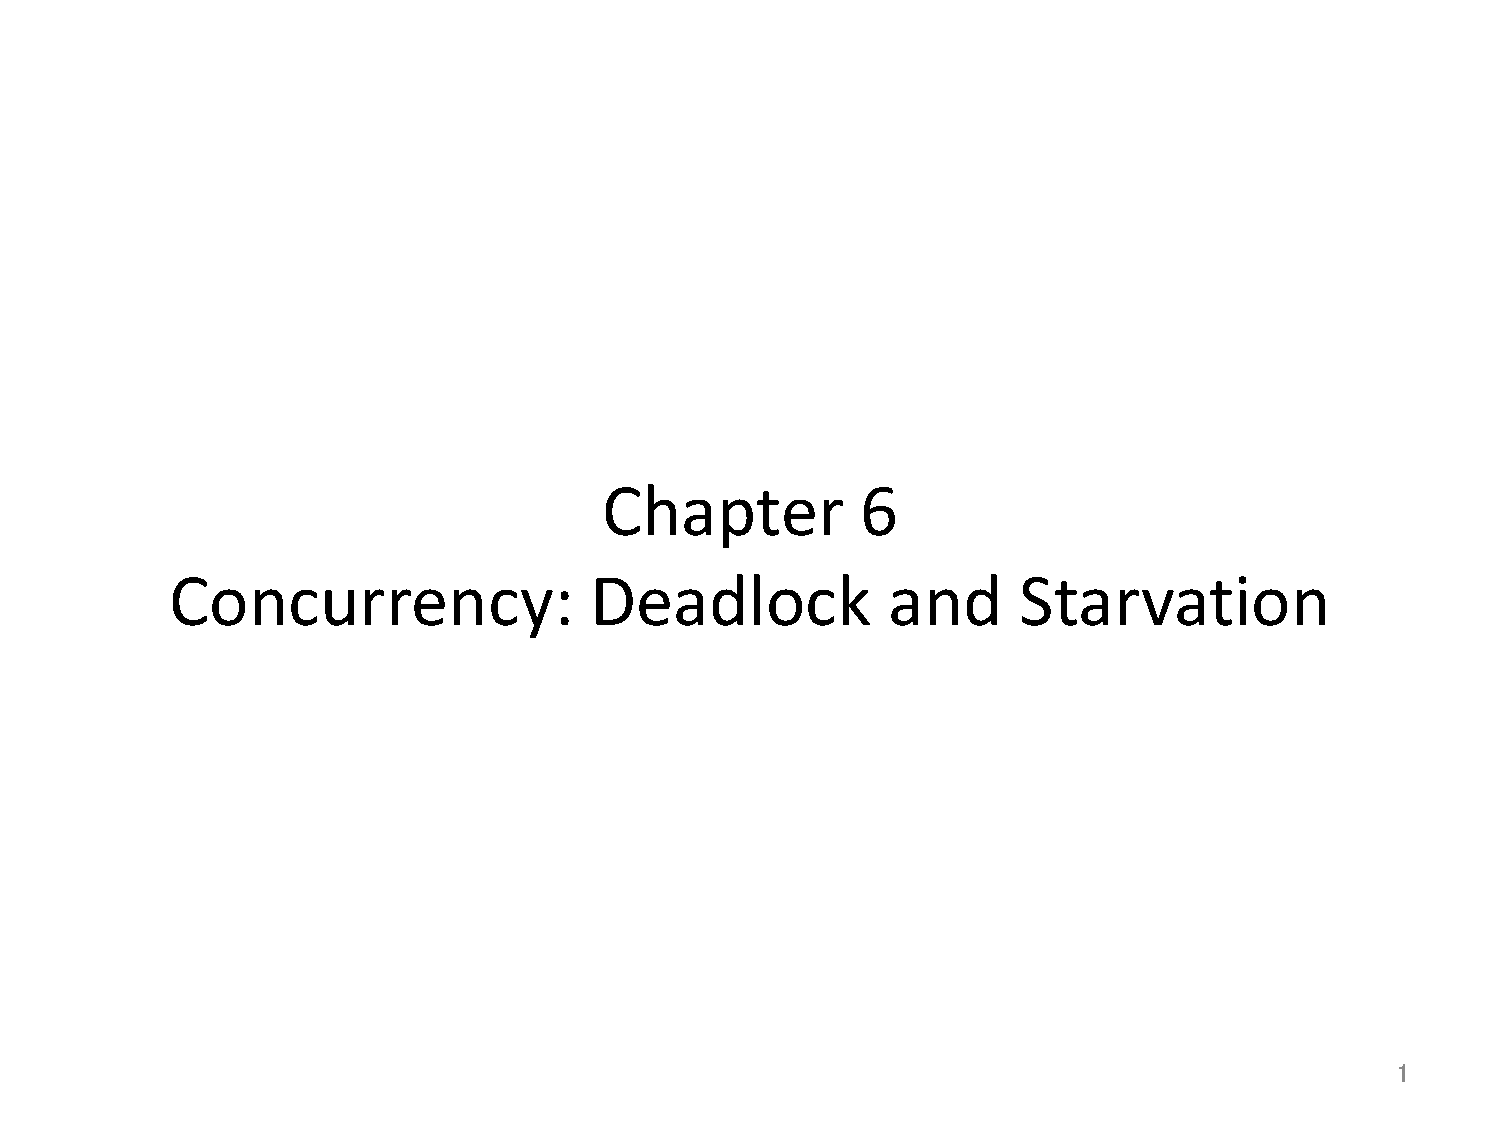
\includepdf[page=19]{06.pdf}
Make a descision based on if a process should be started. Requires upfront knowledge of what resources are required by that resource (R). Need to keep track of the unallocated resources (V). C (claim matrix) keeps table of processes and the total resources they will need (processes down, resources across) with claims. A (allocation matrix) keeps table of processses and resources allocated to them (process down, resource across) with allocations. We have m processes and n resources, so $C_{mn}$ is the max allocation of $R_n$ to $P_m$ and $A_{mn}$ is current allocation of $R_n$ to $P_m$.

Rules.
\begin{enumerate}
    \item  $R_i = v_j + \sum A_{ij}$
    \item $C_{ij} = \leq R_j$
    \item $A_{ij} \leq C_{ij}$
\end{enumerate}

Disadvantages
\begin{itemize}
    \item fixed number of resources (doesnt work for consumable resources)
    \item must state max resources upfront which many processes dont know at their start
    \item independent processes (doesnt account for processes that must wait on each other)
    \item no processes terminating while holding resources
\end{itemize}

Dont start process if $C_{(n+n)} + \sum C_{ij} > R_j$ basically dont start the process if it requires resources that are already in use.
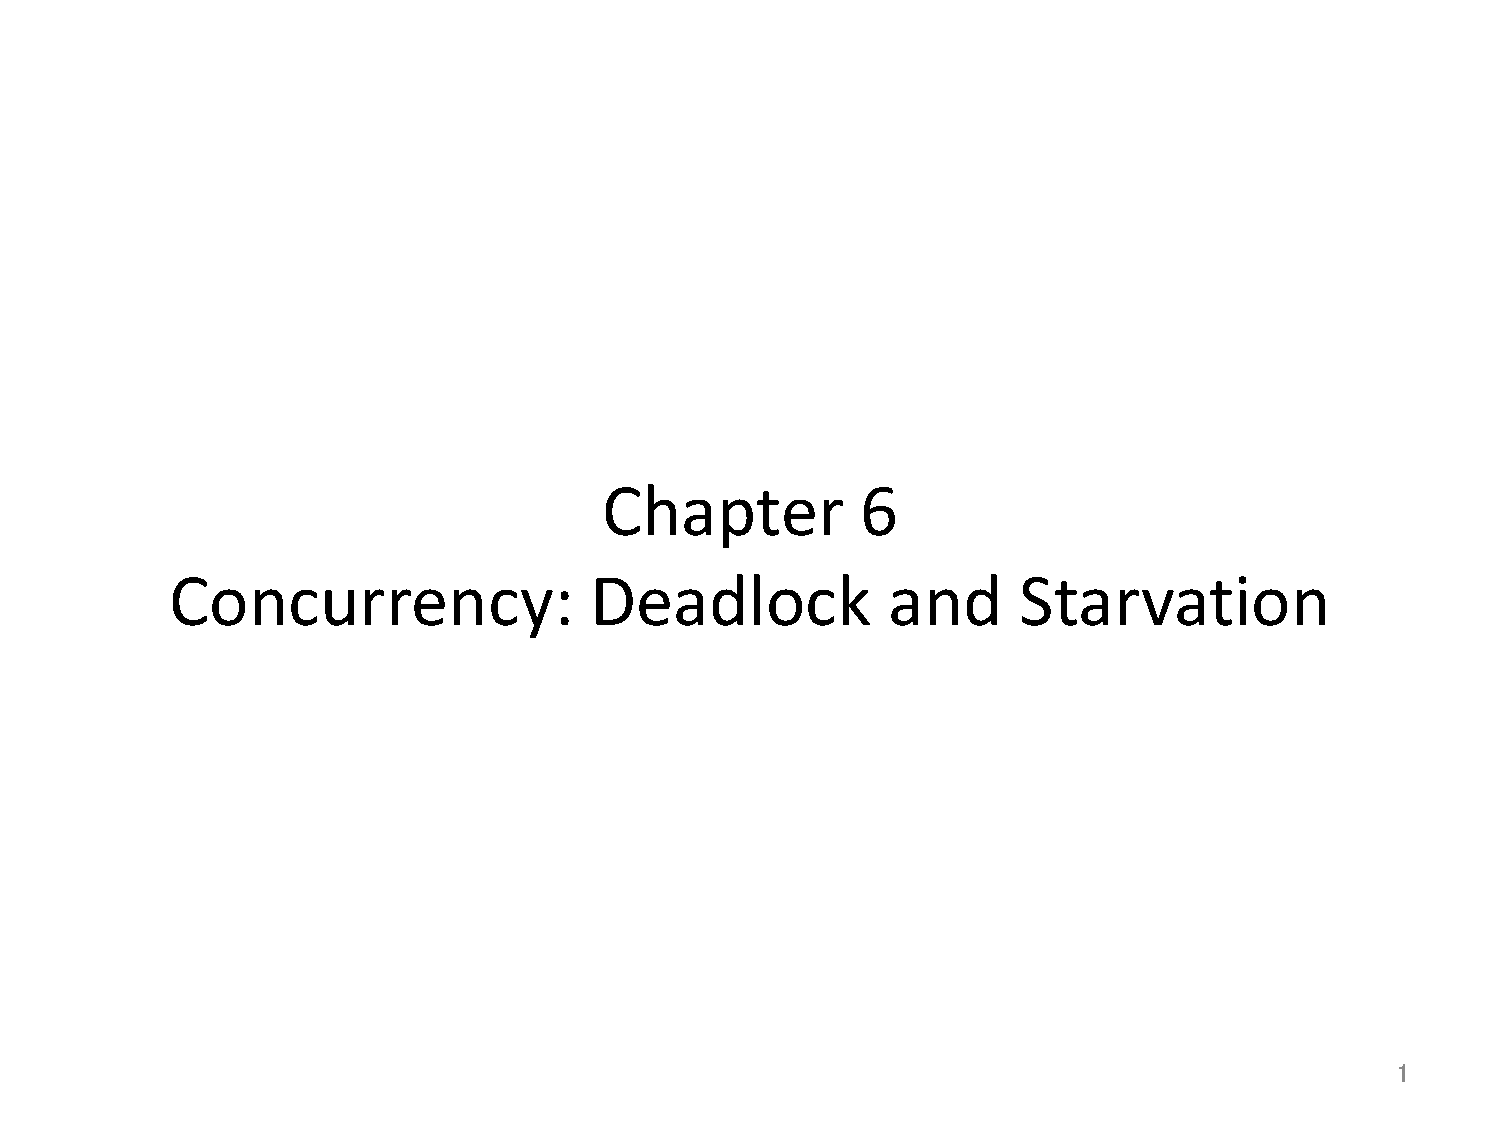
\includepdf[page=20]{06.pdf}
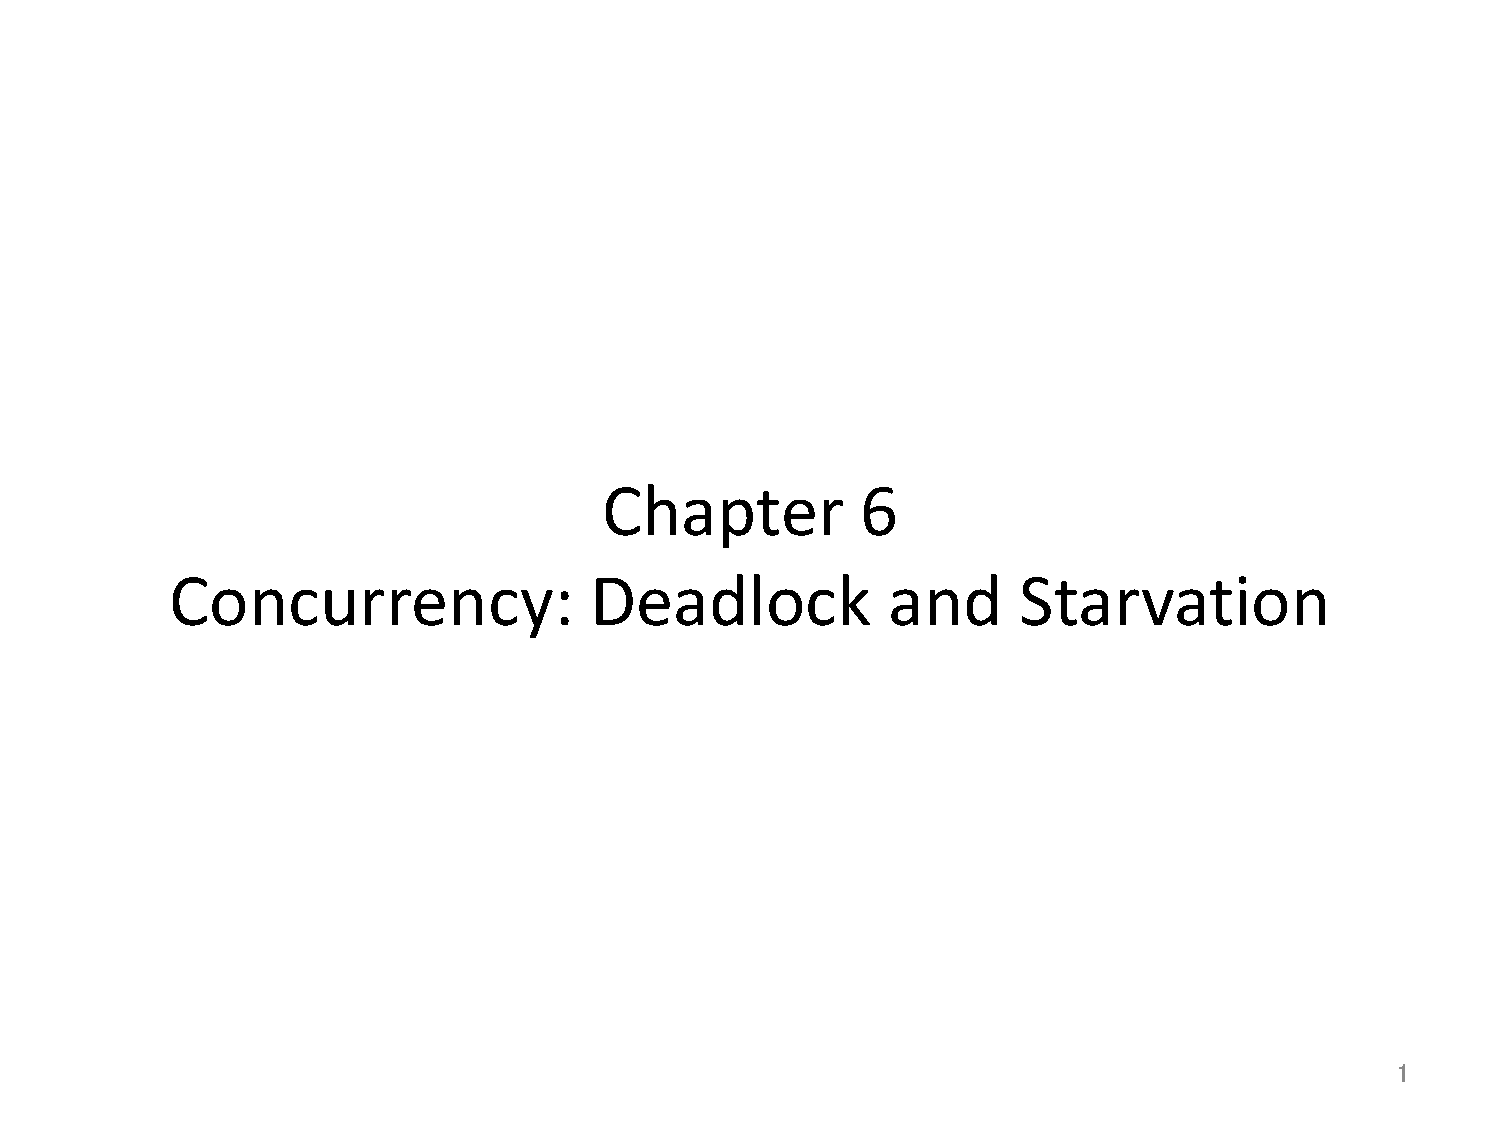
\includepdf[page=21]{06.pdf}
Every time you make a resource request you update matrices and keep going to the end to see if you have a safe state (all allocation are cleared).

ex) The only process we can start with is $P_2$ because the available vector v shows what is available and the matrix c-a show what each process will request, only process two is cleared. So we run process two to completion.
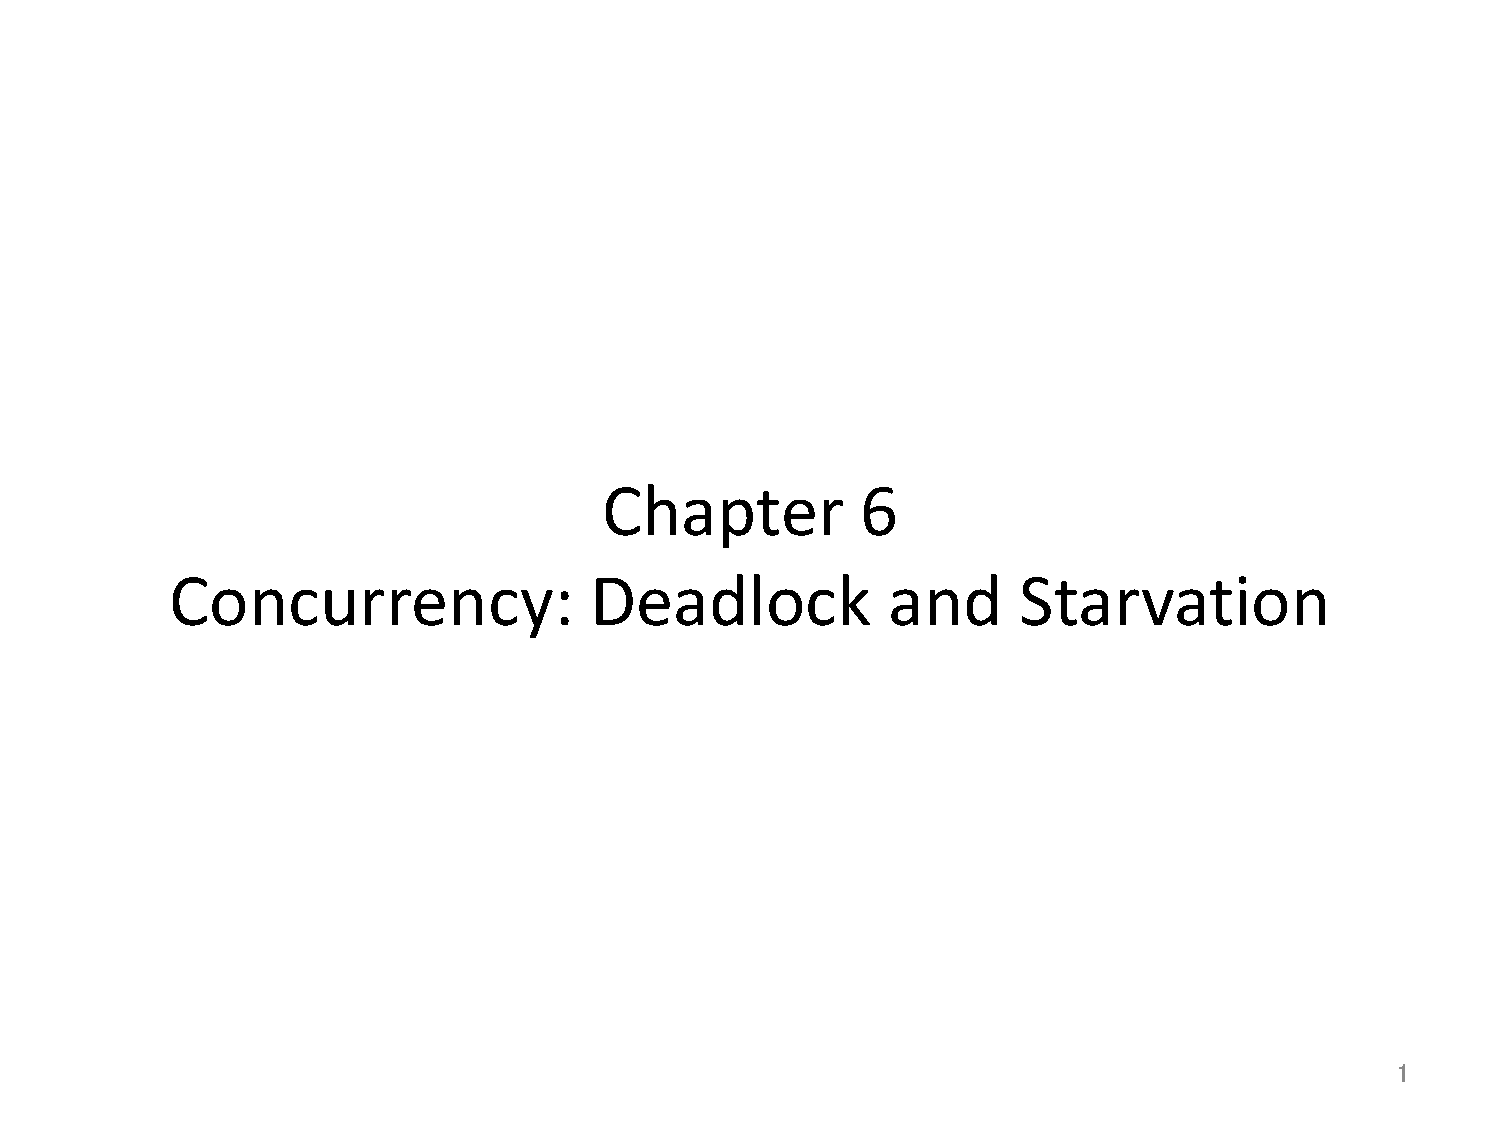
\includepdf[page=22]{06.pdf}
Here every resource allocated to $R_2$ get put on the available vector and update its row in c-a.

Now we can run any program. We repeate this process until we see that every process can execute completely so we know we have a safe state.
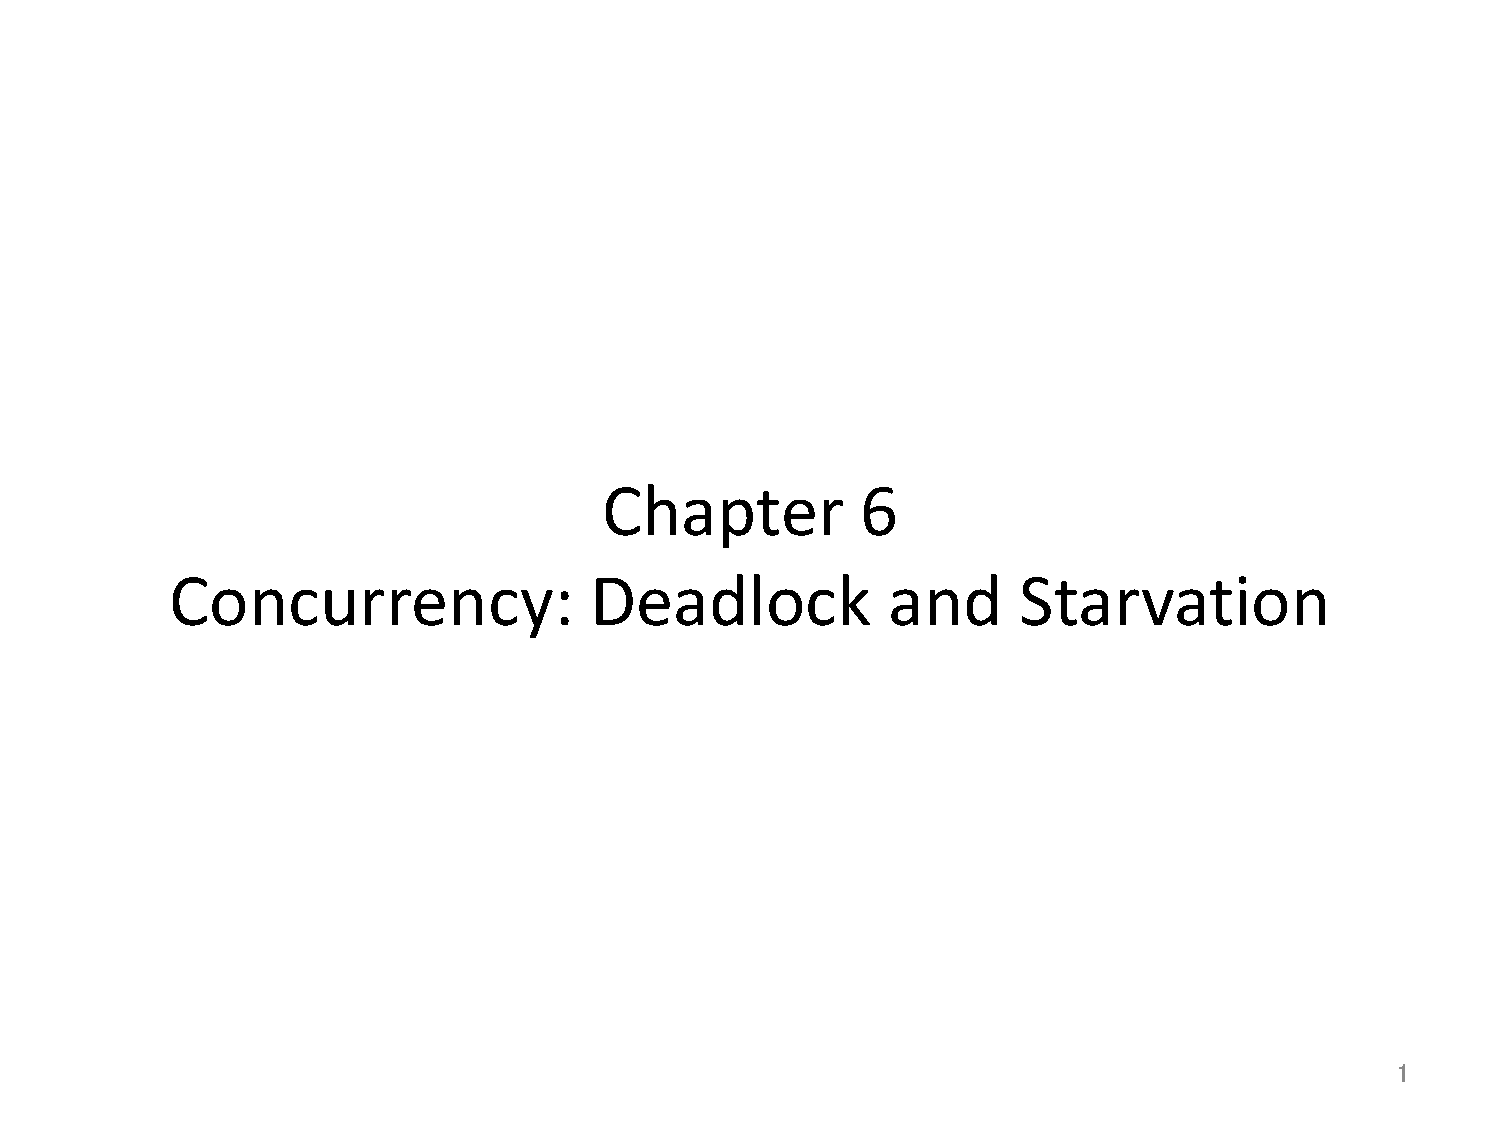
\includepdf[page=23]{06.pdf}
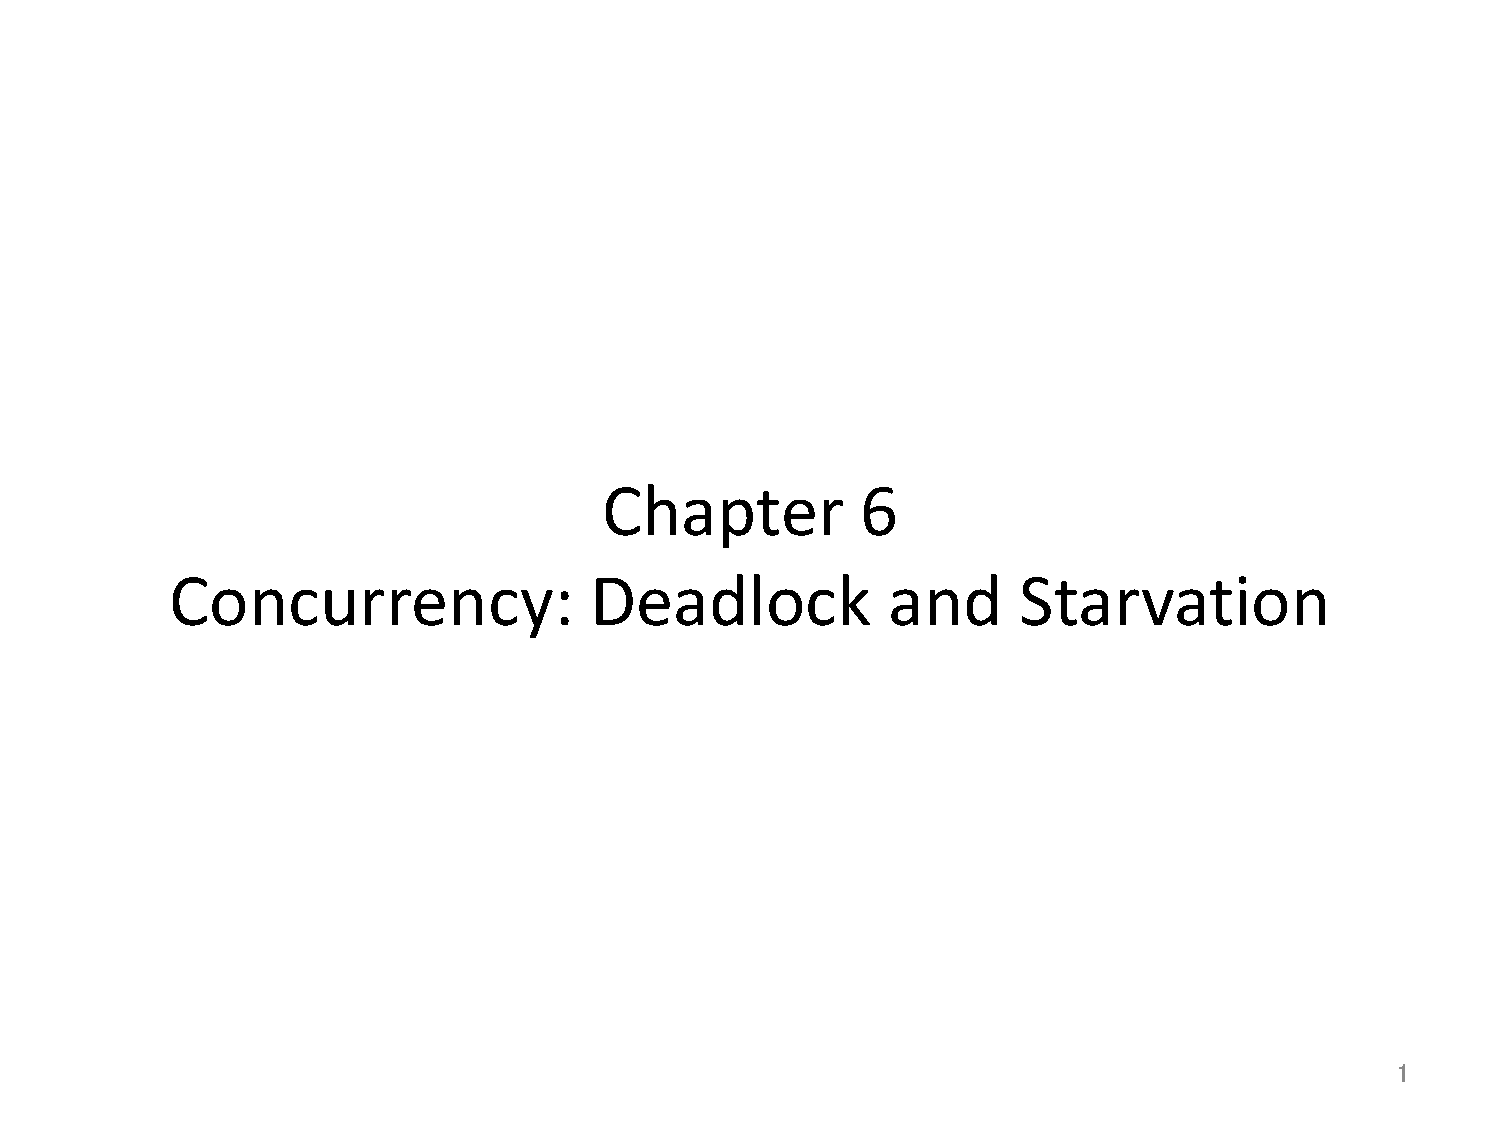
\includepdf[page=24]{06.pdf}
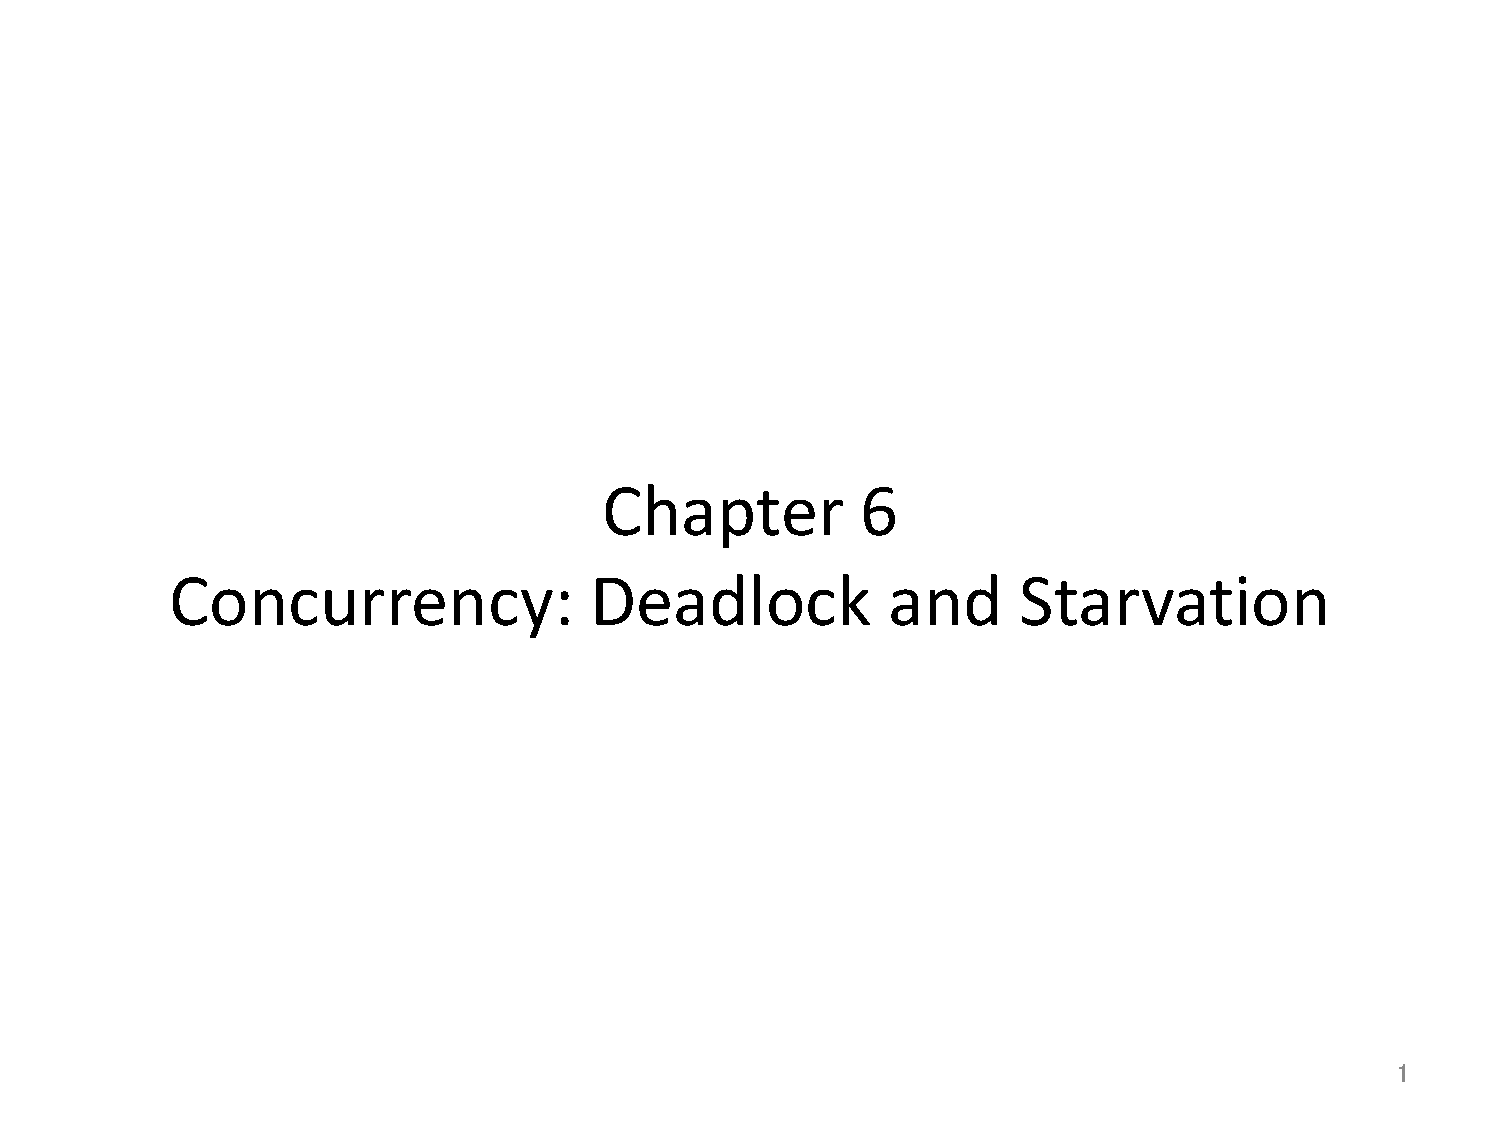
\includepdf[page=25]{06.pdf}
We see here from the initial state the the only process we can run is $P_2$ making available = [0,1,1] (we took the incremental resources 1 x $R_1$ and 1x $R_3$ away to allocate them to $P_2$). This step is done because of incremental allocation (we dont go to termination and return the resources instead we try to start a new process between incremental allocations). Now we cannot start any process safely, called a unsafe state.
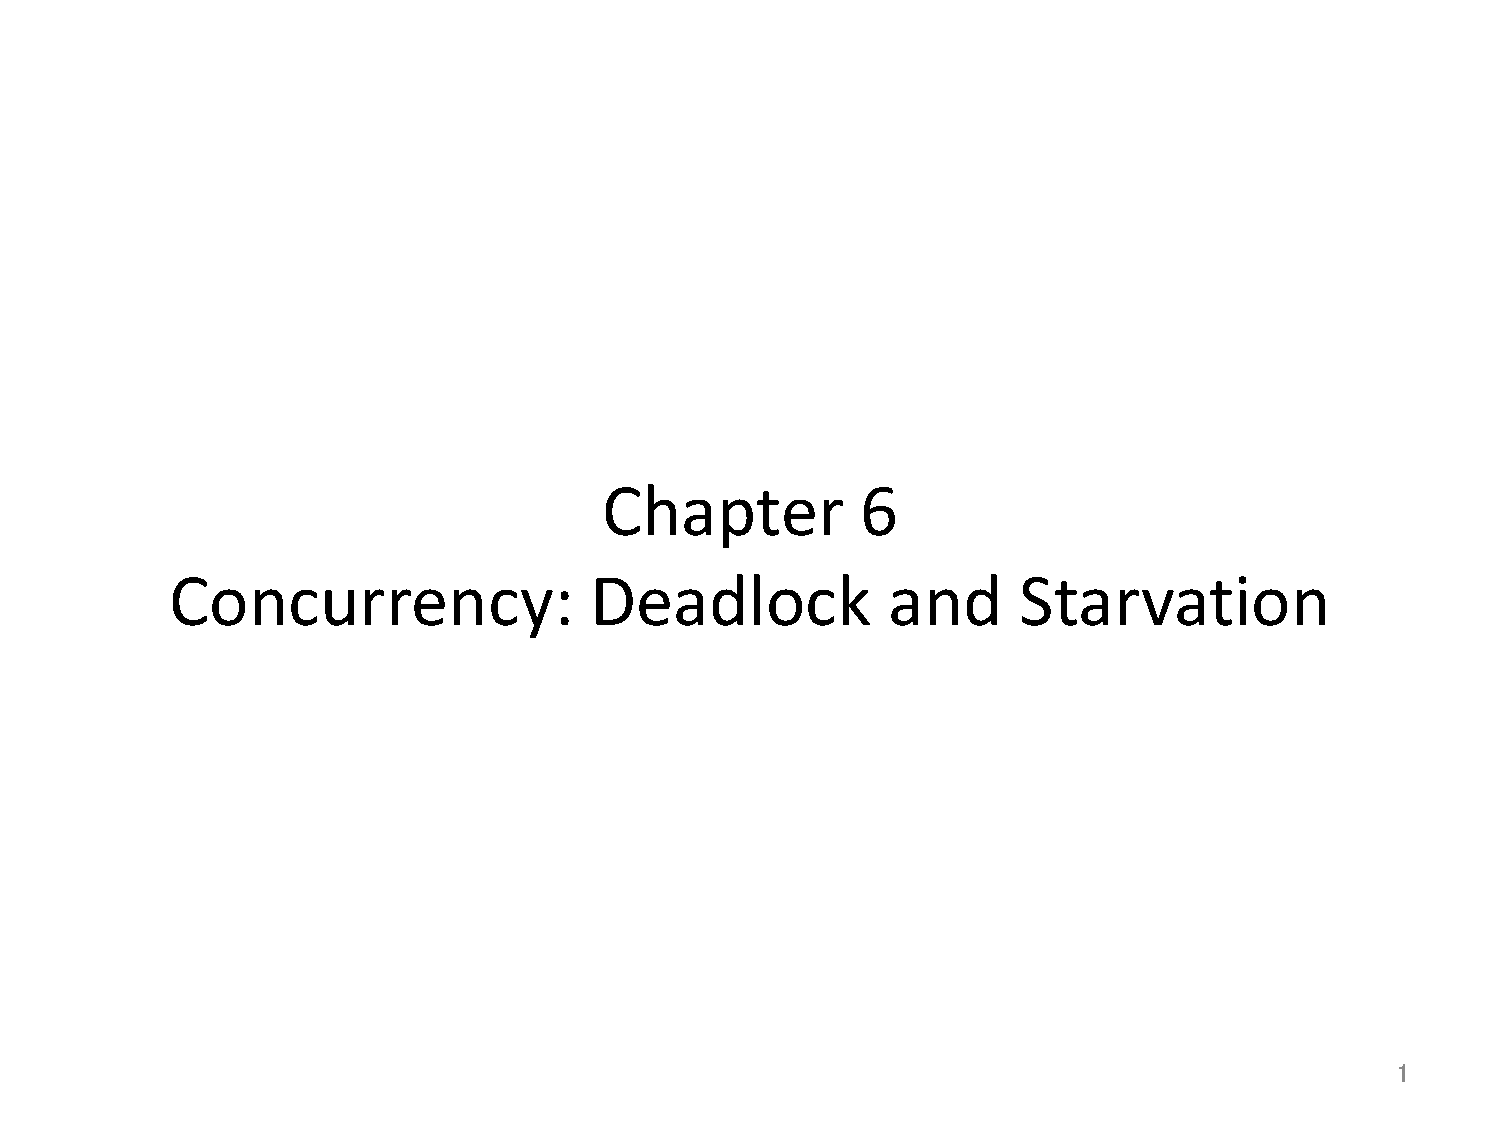
\includepdf[page=26]{06.pdf}
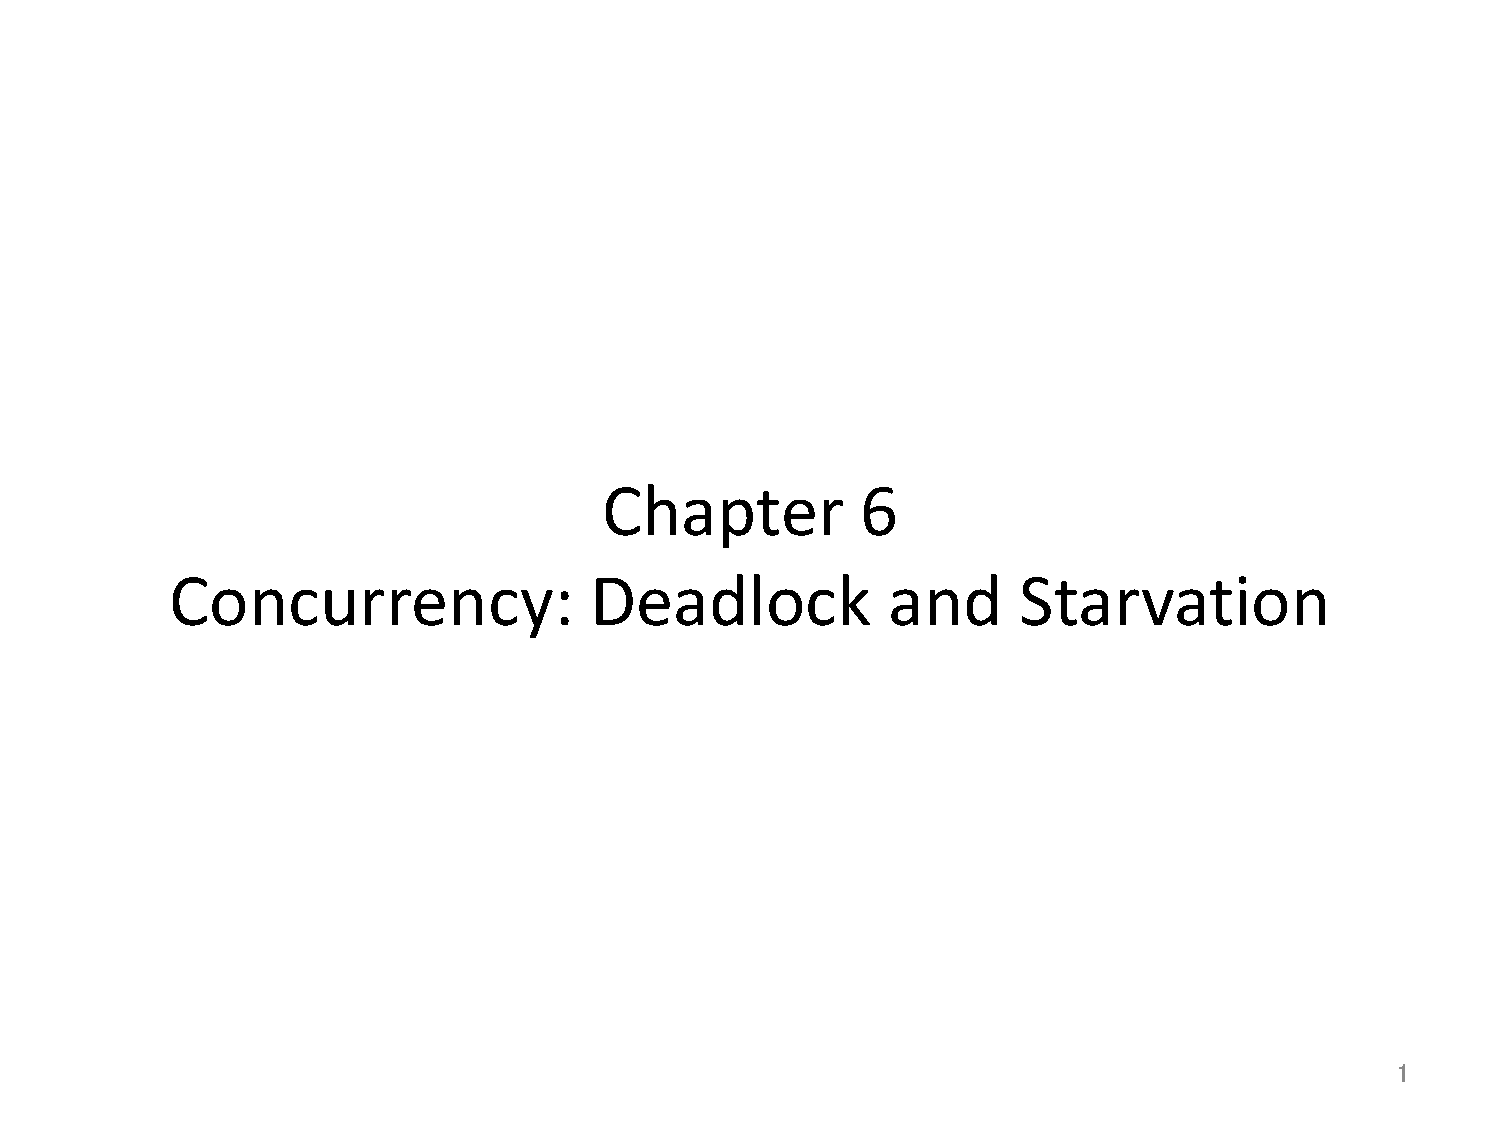
\includepdf[page=27]{06.pdf}
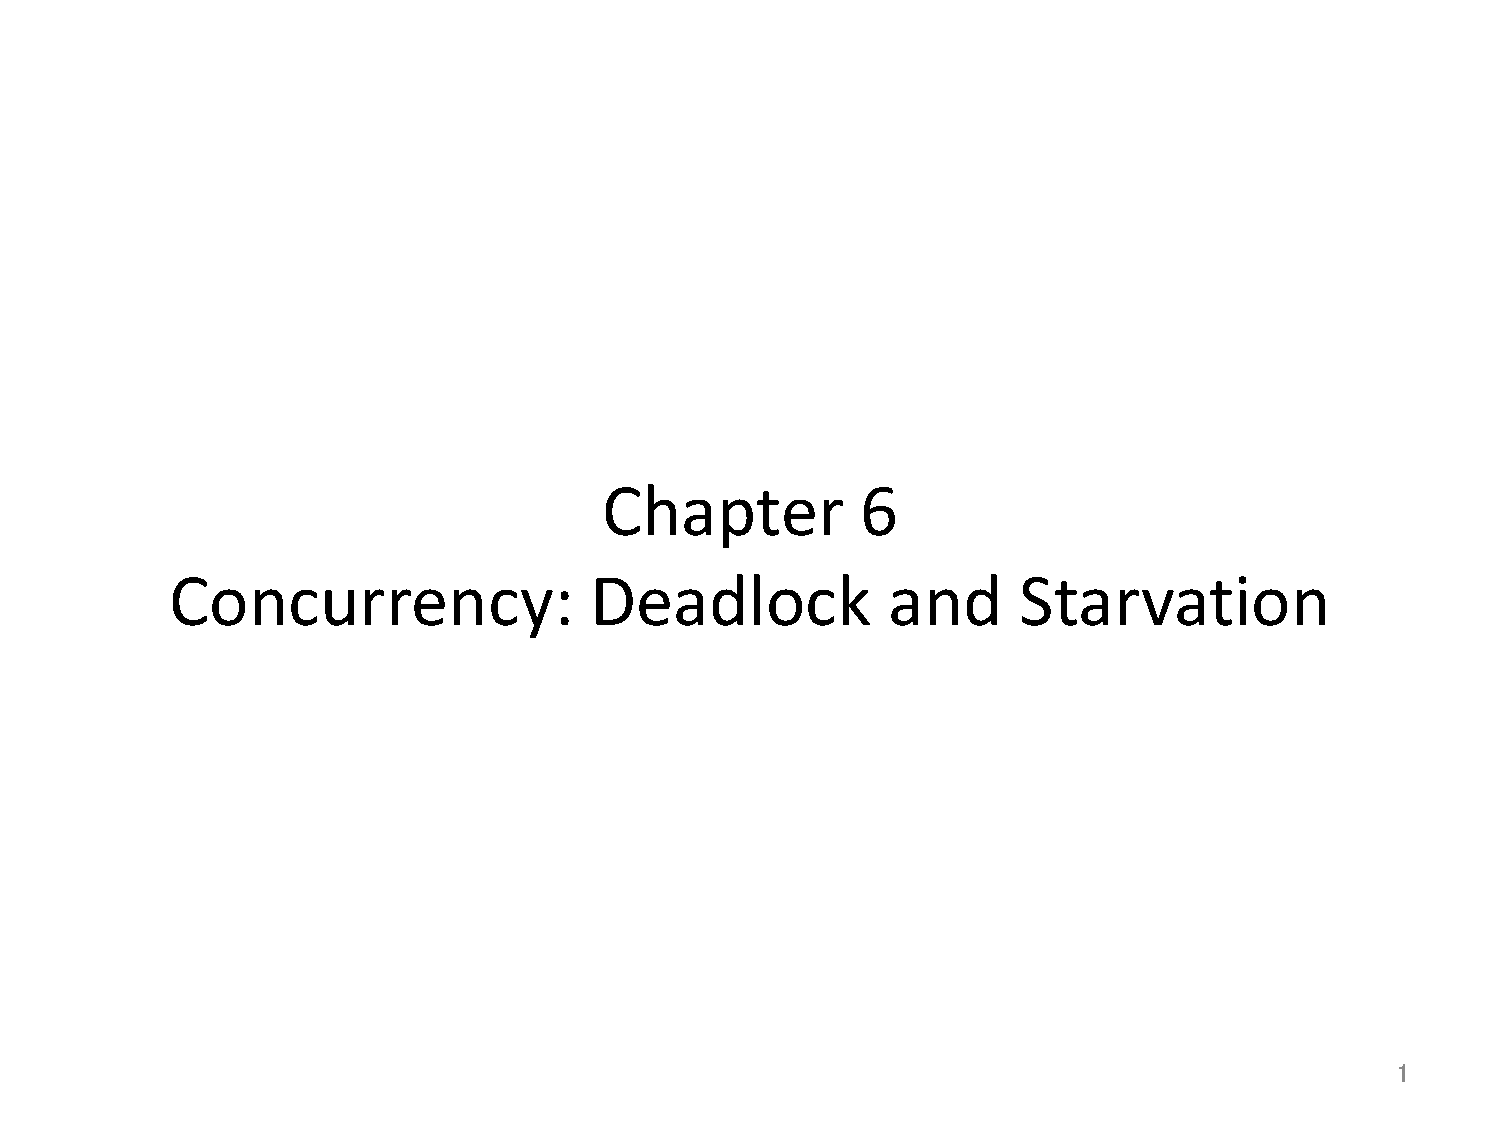
\includepdf[page=28]{06.pdf}
To use the baker We algorithm we need to fit the above criteria.
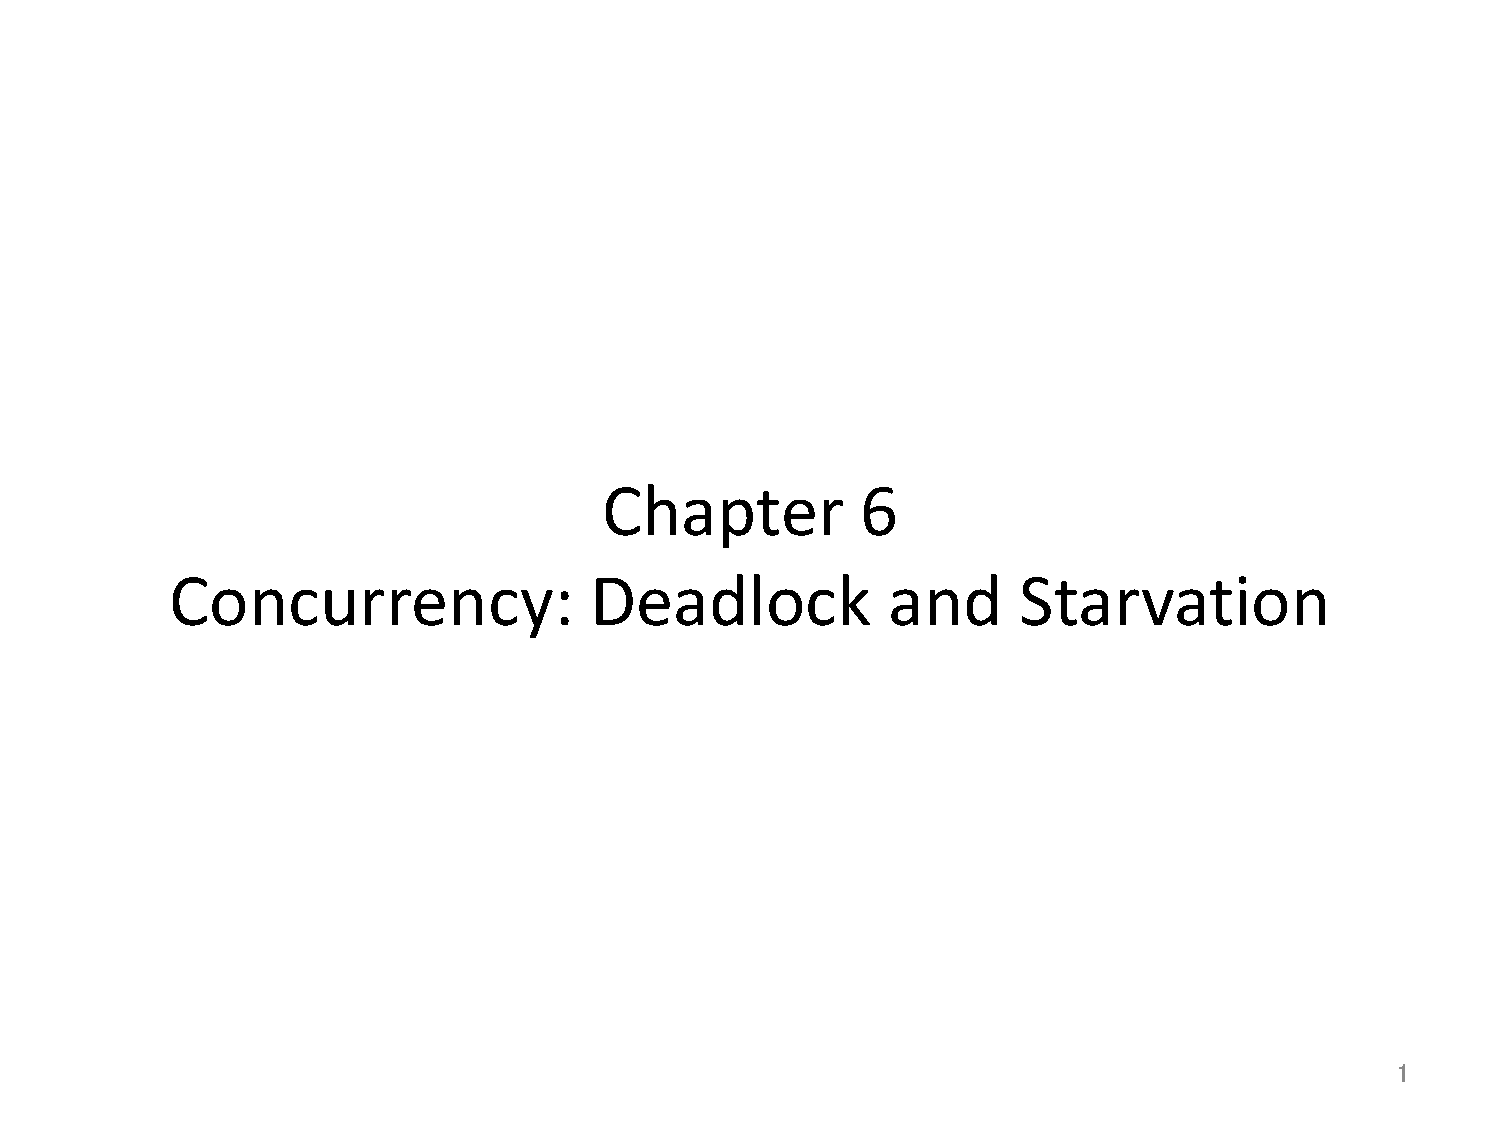
\includepdf[page=29]{06.pdf}
We model outstanding requests using a simplified version (Q = C - A at that instant) seen above. Now we run the same algorithm as last time. Want to find if deadlock and look for processes that can be deadlocked.

\begin{itemize}
    \item mark all processes that have no resources allocated.
    \item w := V  initialize to available vector
    \item look for a process that you can satisfy (room in available vector for values in Q), these are not in a deadlock state
    \item release all resources in available vector (like running to completion)
    \item repeat for all processes (unless a deadlock is reached)
\end{itemize}
Applied methodology of bankers algorithm but removed the need to state all required resources at the start. With this we can mock deadlock transactions before letting them run through.
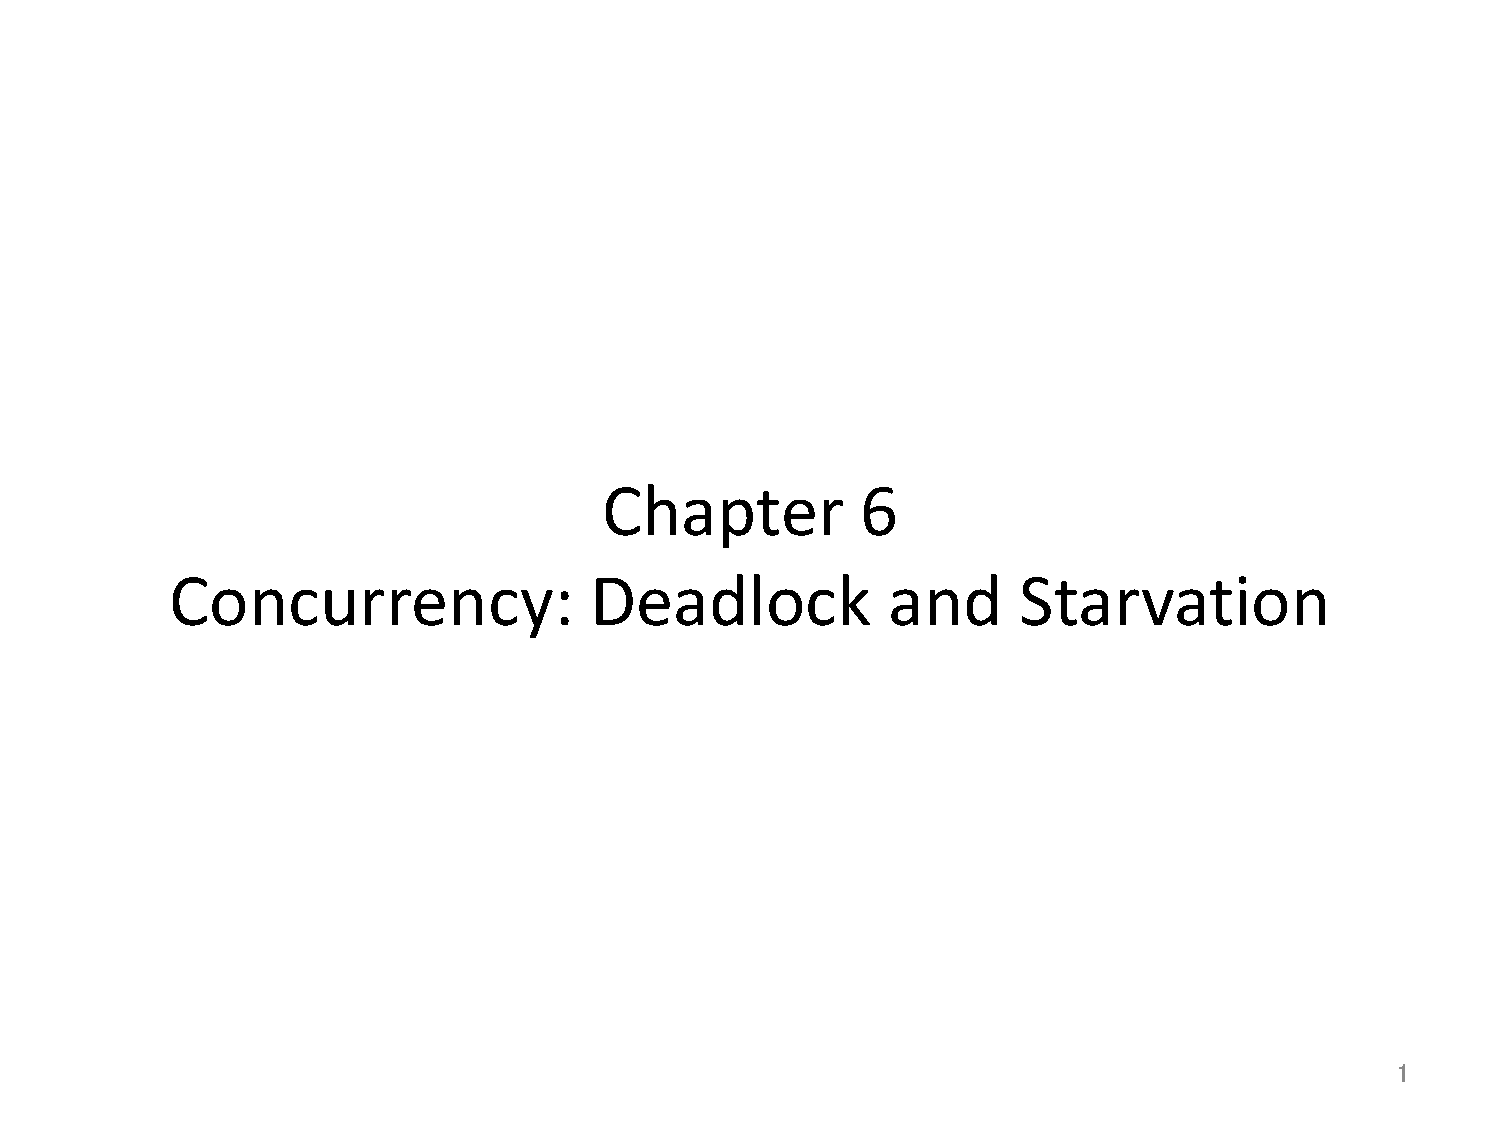
\includepdf[page=30]{06.pdf}
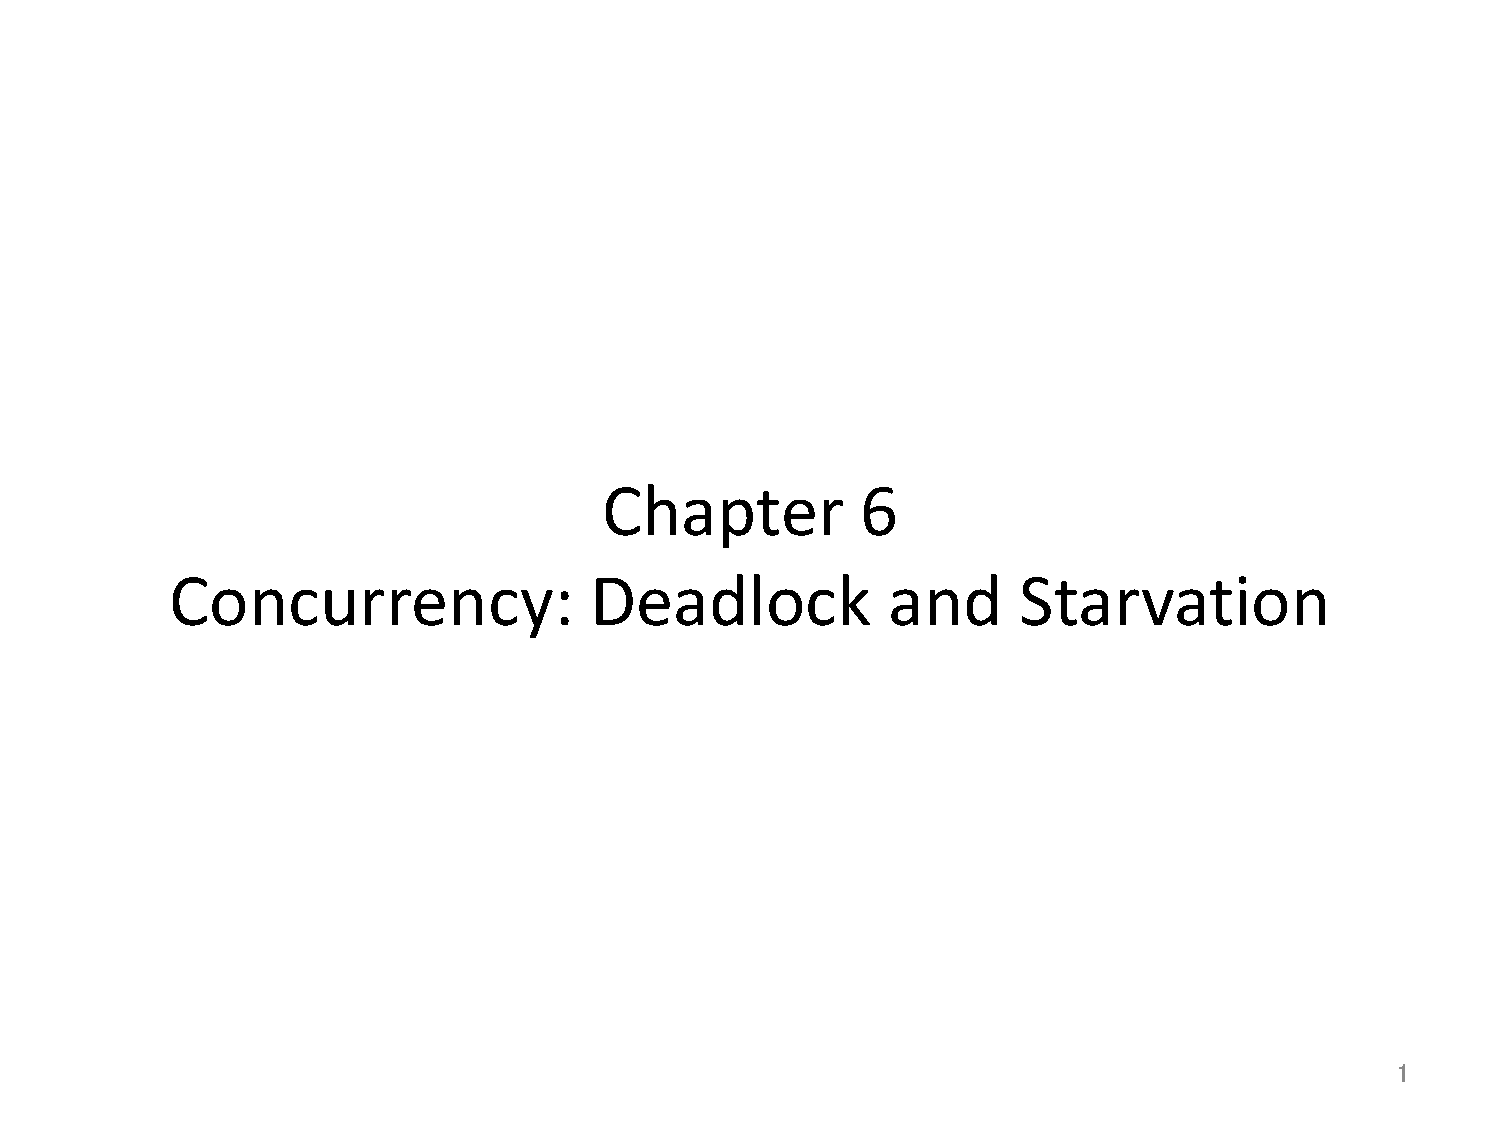
\includepdf[page=31]{06.pdf}
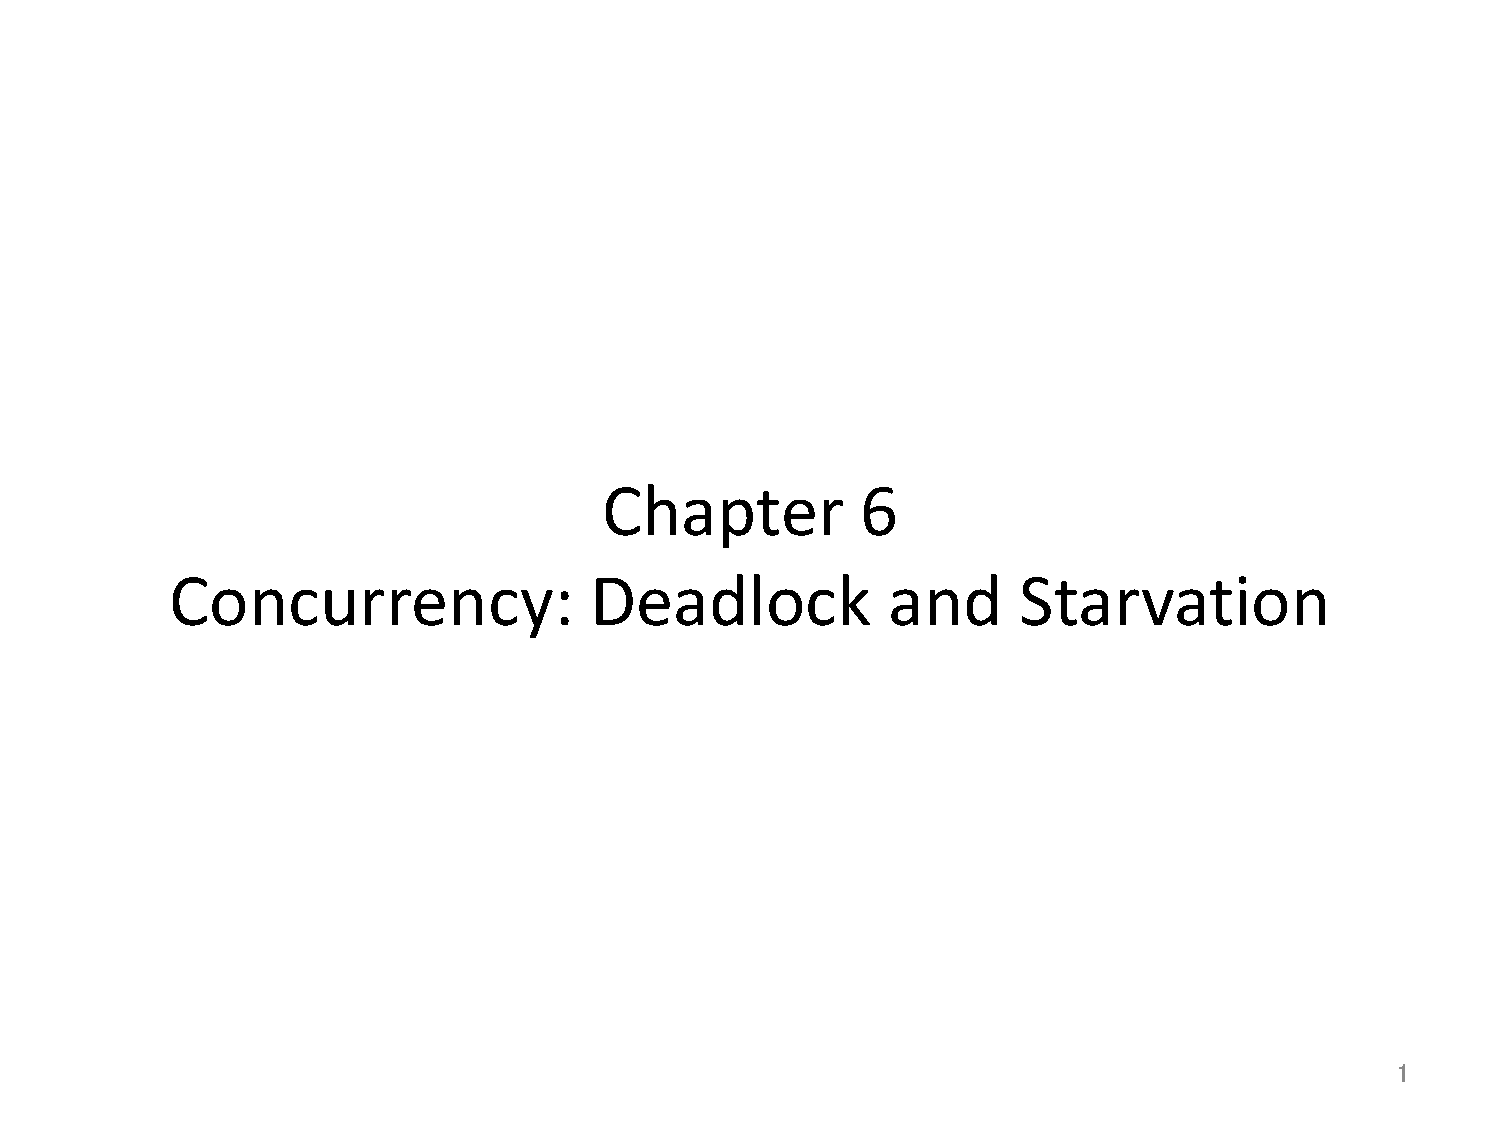
\includepdf[page=32]{06.pdf}
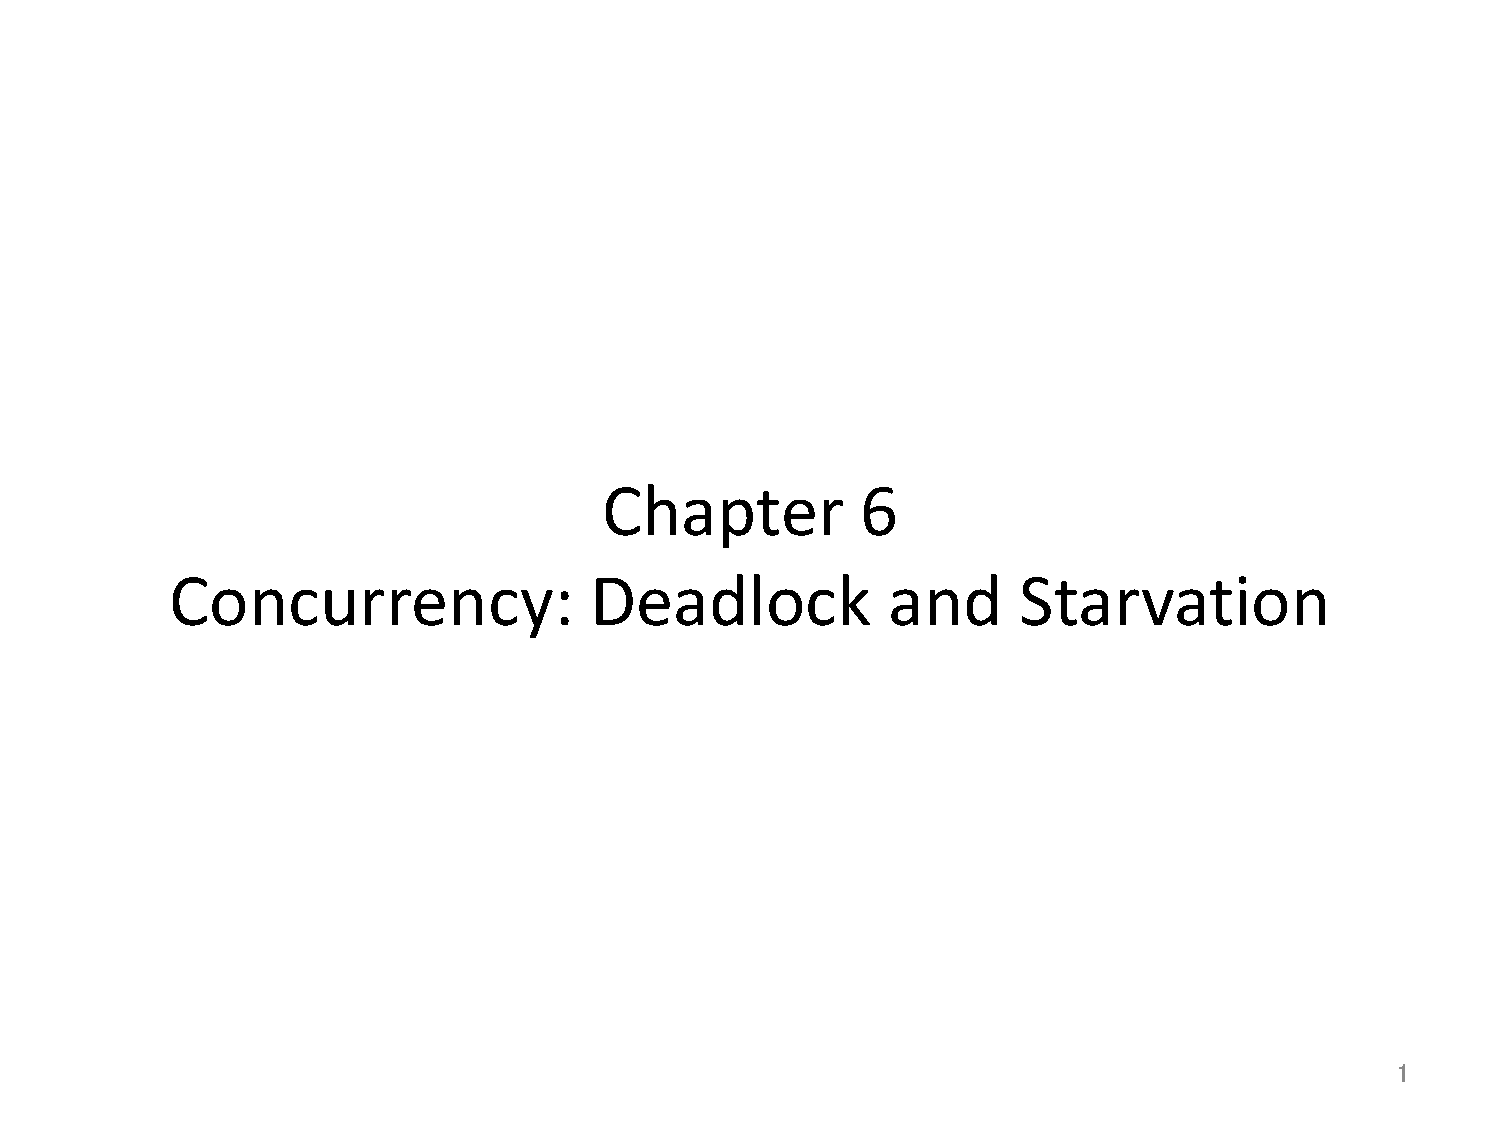
\includepdf[page=33]{06.pdf}
A deadlock is reached when every philosopher wants to eat at the same time.
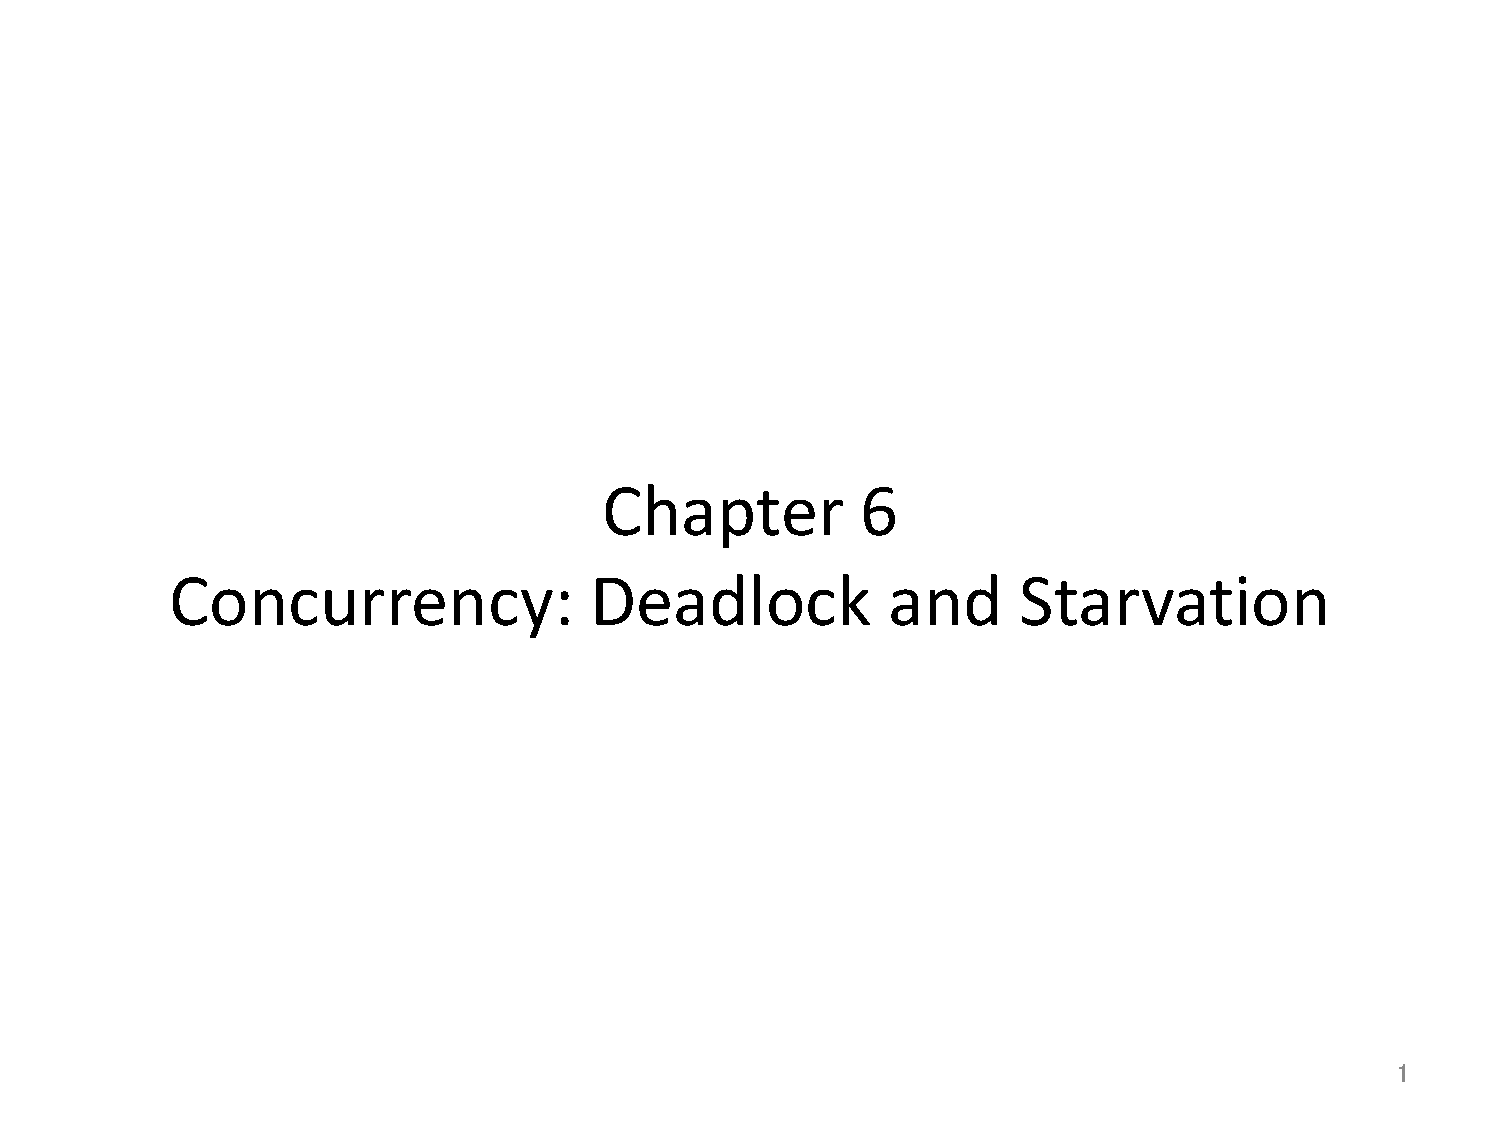
\includepdf[page=34]{06.pdf}
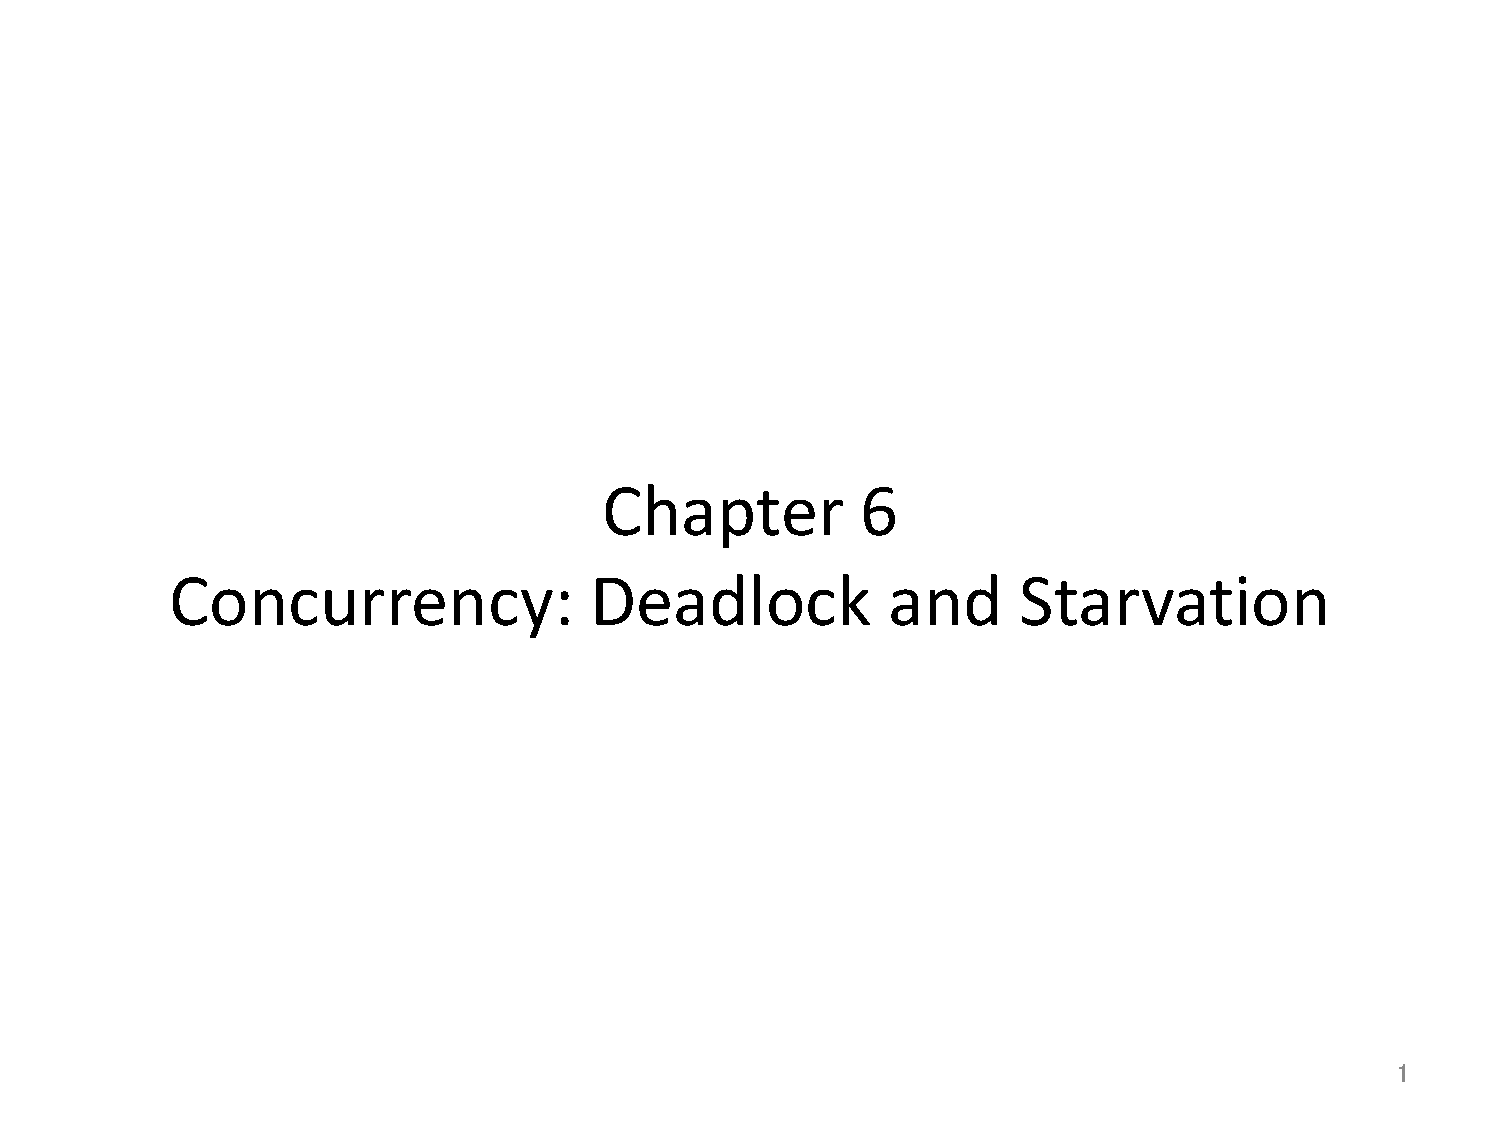
\includepdf[page=35]{06.pdf}
One solution is to have a bouncer that only allows four people in at a time. We can do this by wrapping the logic or the philosophers in a semaphore that only allows four in at a time.
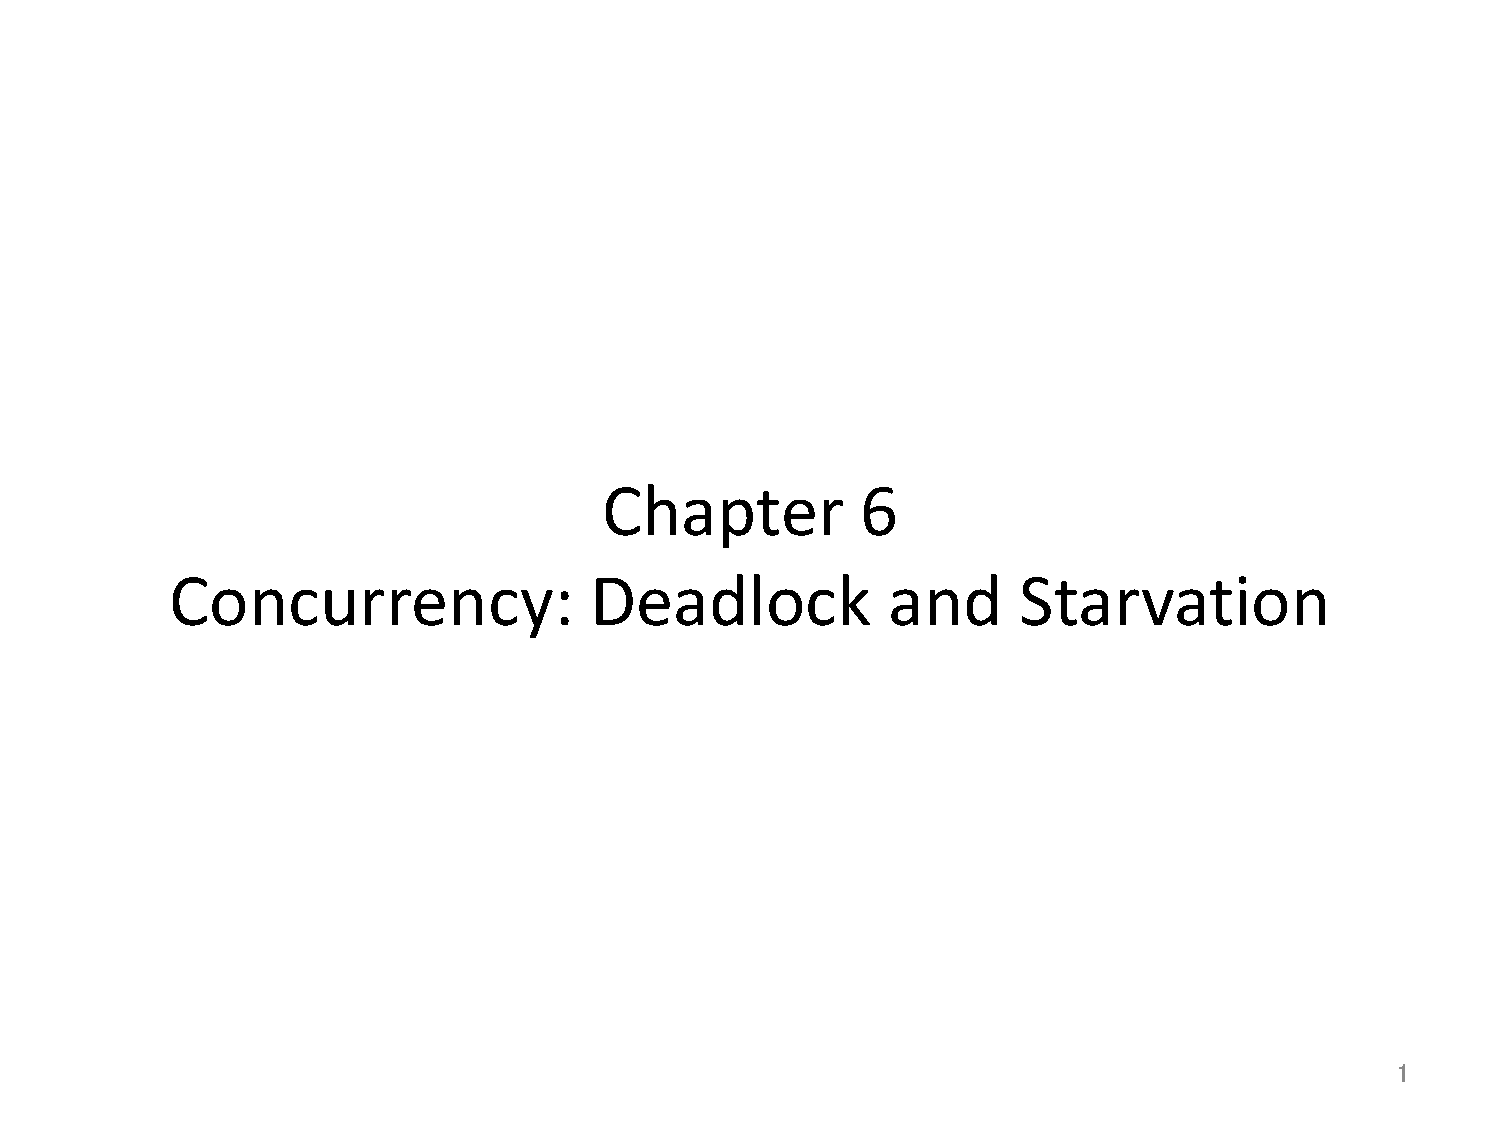
\includepdf[page=36]{06.pdf}
This is the monitor solution. Wrap get forks and release forks in it. When someone wants to pick up a fork you check for availability for the left fork and right fork and signal for availability.
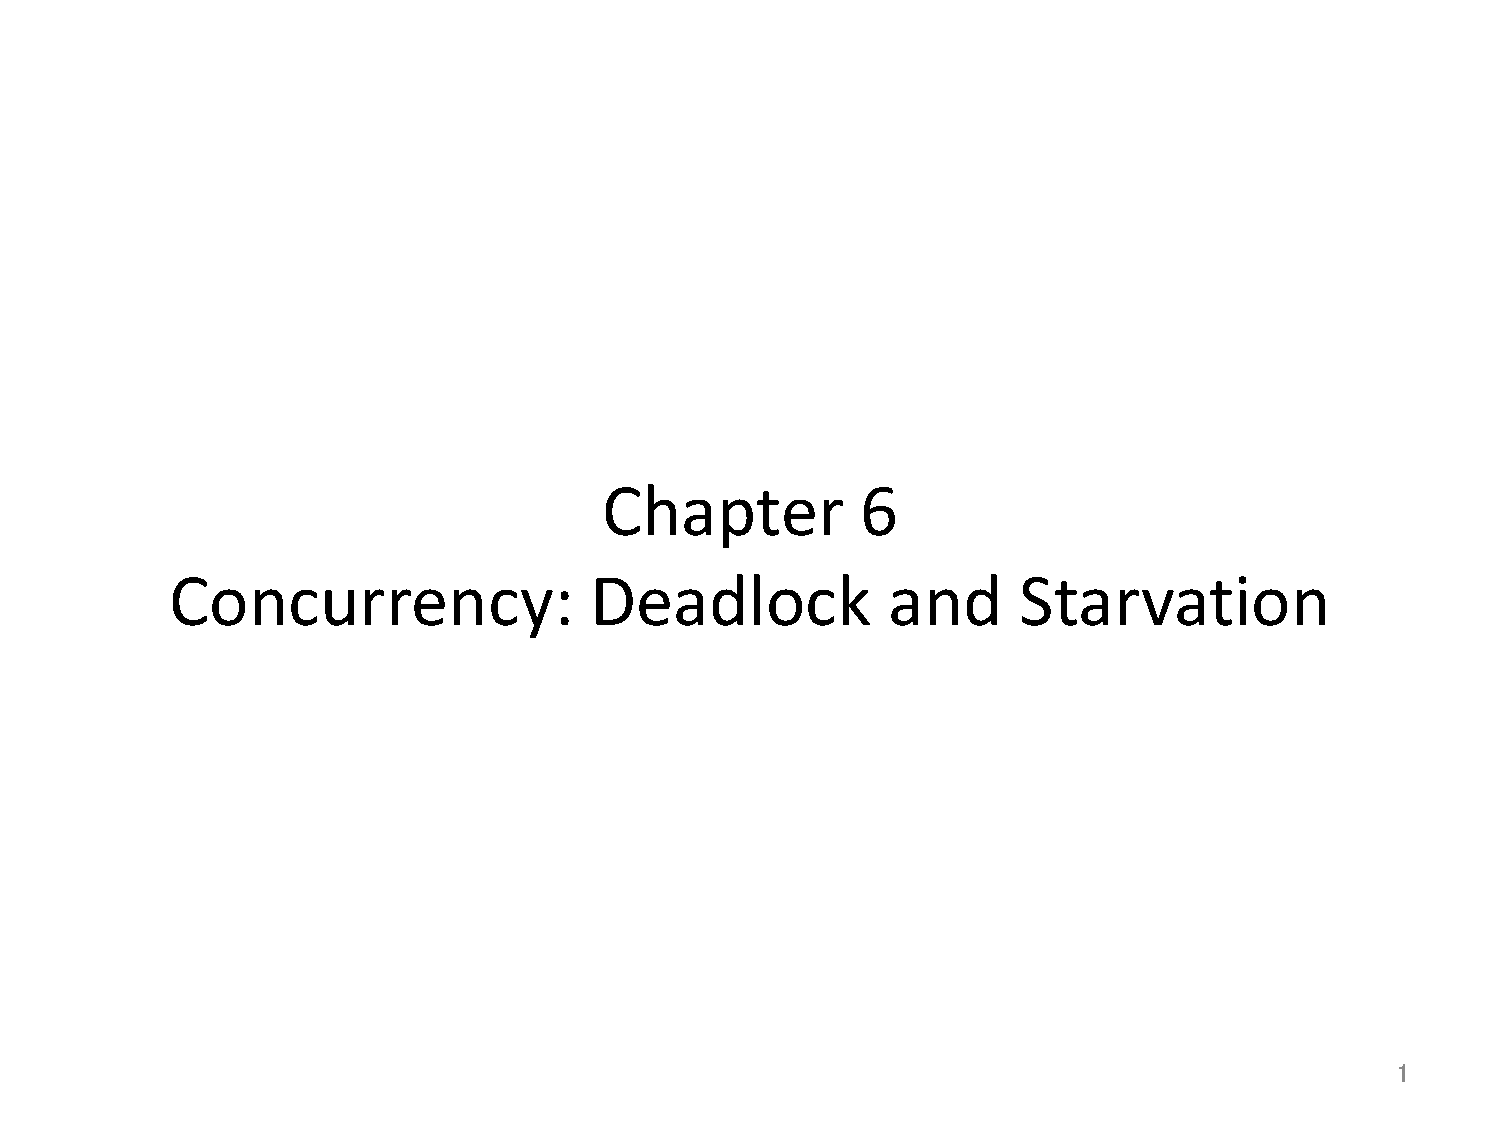
\includepdf[page=37]{06.pdf}
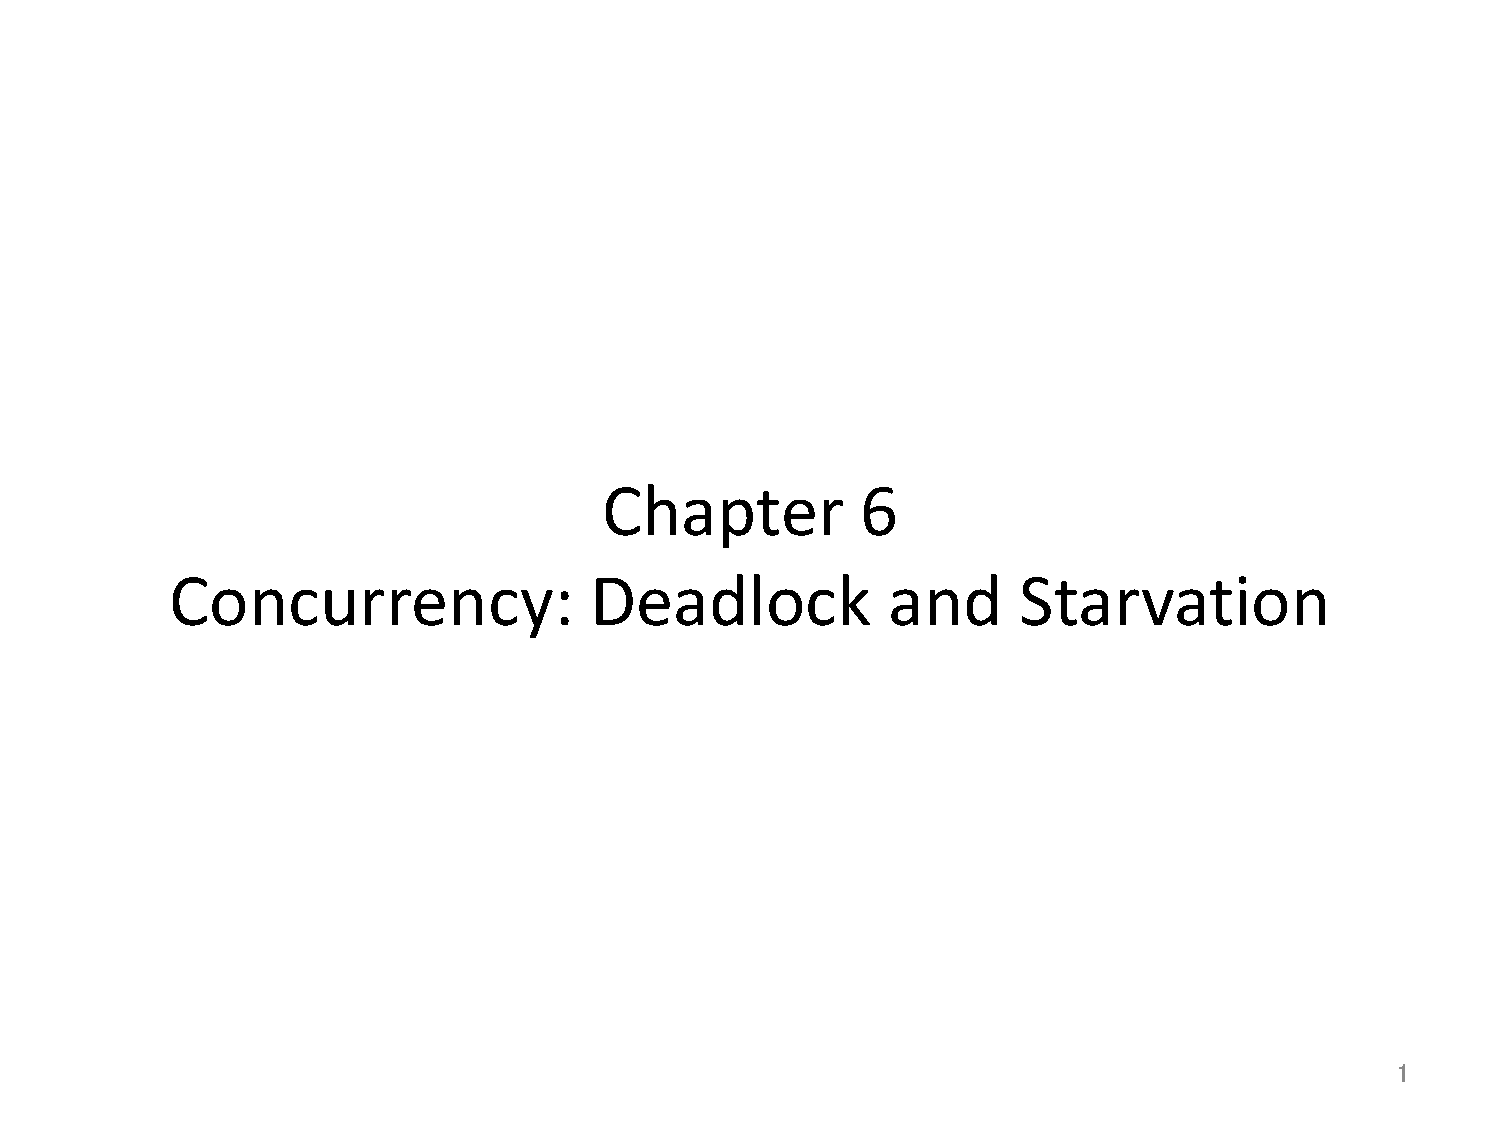
\includepdf[page=38]{06.pdf}
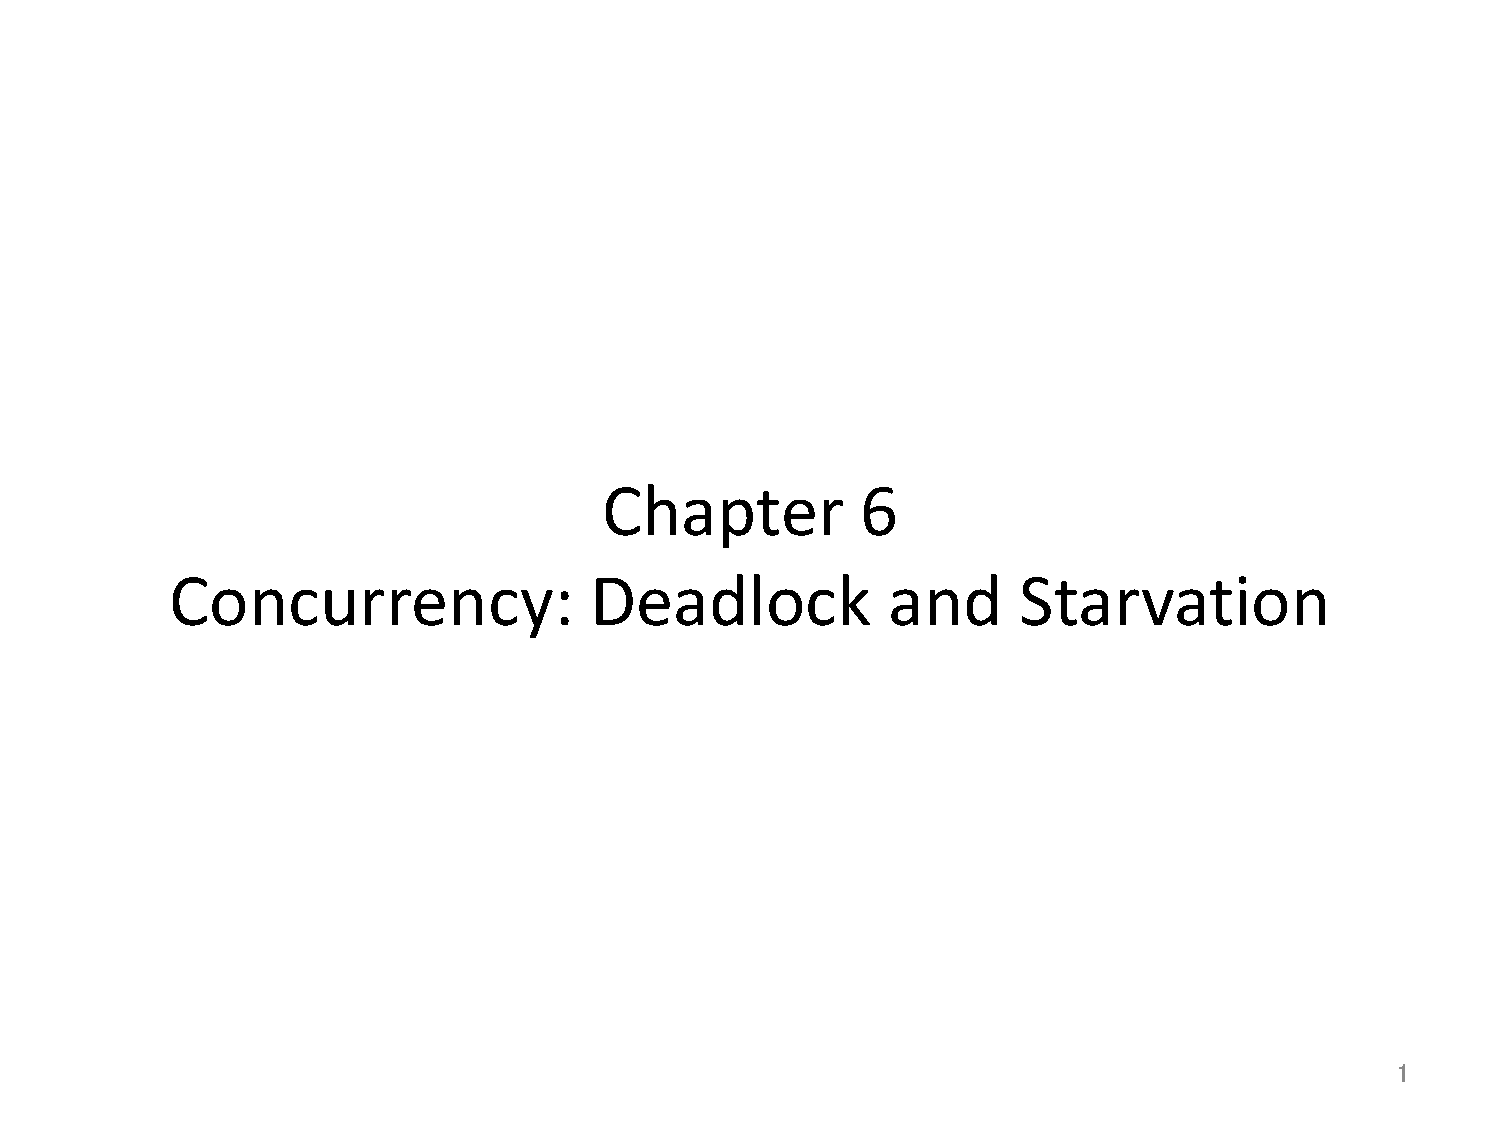
\includepdf[page=39]{06.pdf}
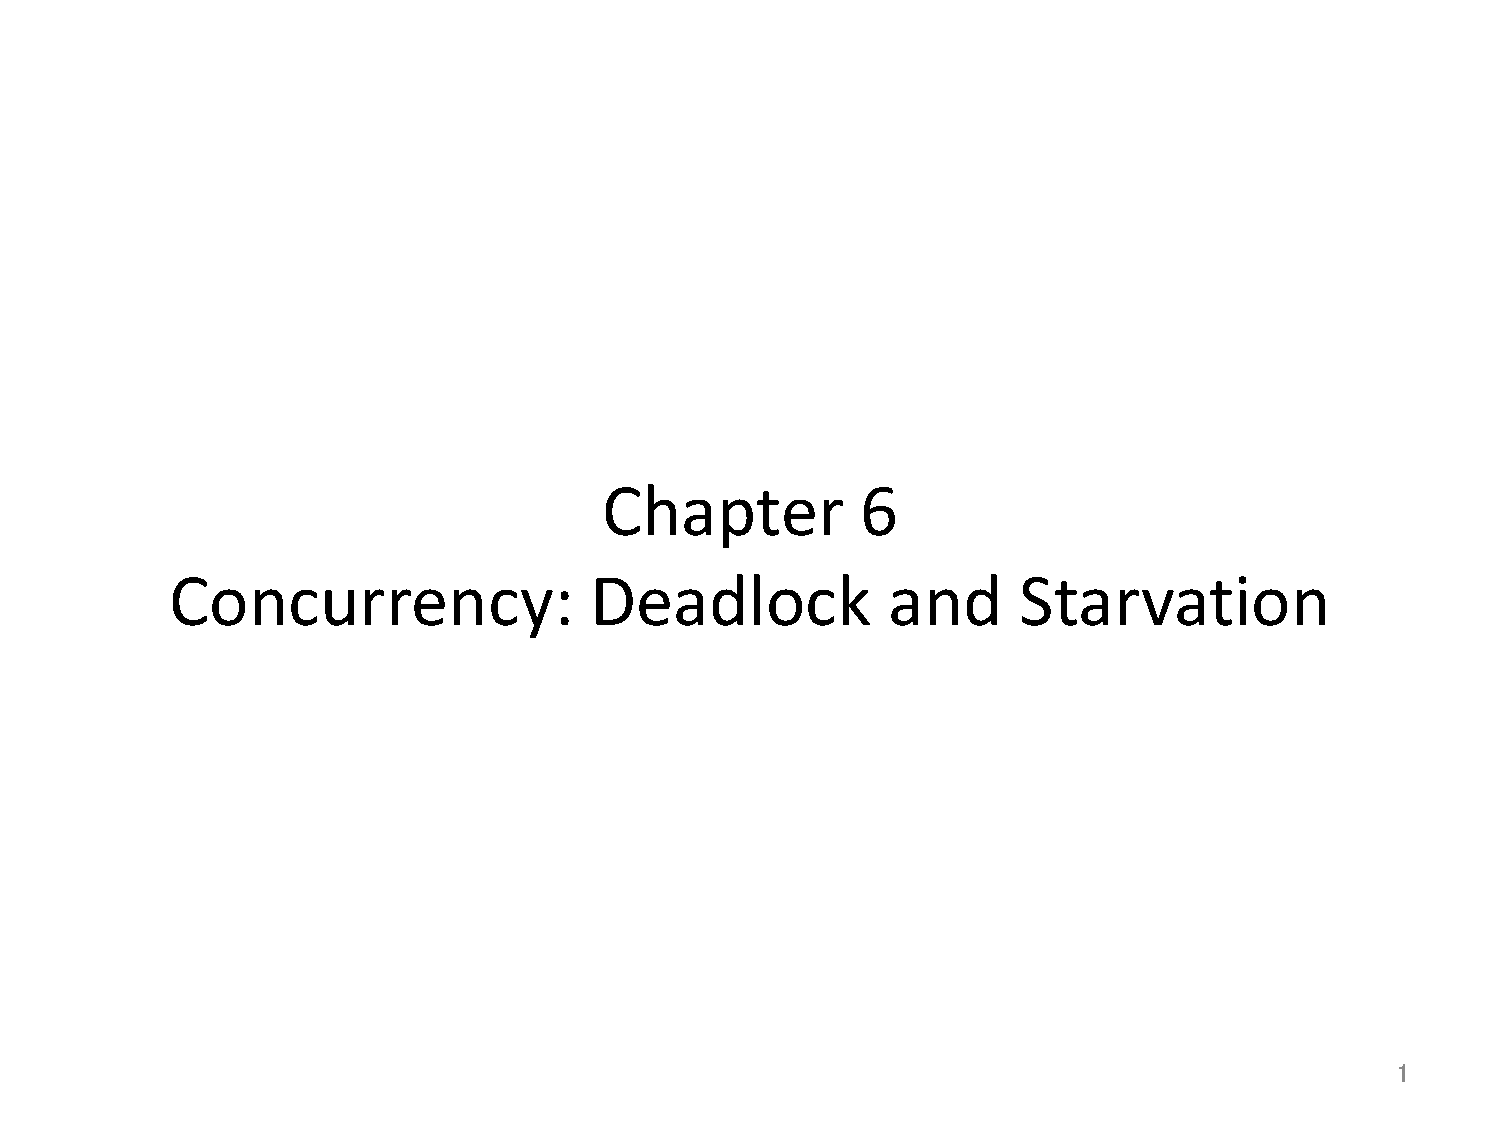
\includepdf[page=40]{06.pdf}
\end{document}
